\documentclass{article}

\usepackage{amsmath, amsthm, amssymb, amsfonts}
\usepackage{thmtools}
\usepackage{graphicx}t

\usepackage{setspace}
\usepackage{geometry}
\usepackage{float}
\usepackage{hyperref}
\usepackage[utf8]{inputenc}
\usepackage[english]{babel}
\usepackage{framed}
\usepackage[dvipsnames]{xcolor}
\usepackage{tcolorbox}


\usepackage{graphicx}

\usepackage{hyperref}
\hypersetup{
    colorlinks=true,
    linkcolor=blue,
    filecolor=magenta,      
    urlcolor=cyan,
    pdftitle={Overleaf Example},
    pdfpagemode=FullScreen,
    }
\urlstyle{same}

% create subsubsubsection command
% see https://tex.stackexchange.com/questions/60209/how-to-add-an-extra-level-of-sections-with-headings-below-subsubsection
\usepackage{titlesec}
\titleclass{\subsubsubsection}{straight}[\subsection]
\newcounter{subsubsubsection}[subsubsection]
\renewcommand\thesubsubsubsection{\thesubsubsection.\arabic{subsubsubsection}}
\renewcommand\theparagraph{\thesubsubsubsection.\arabic{paragraph}} % optional; useful if paragraphs are to be numbered
\titleformat{\subsubsubsection}
  {\normalfont\normalsize\bfseries}{\thesubsubsubsection}{1em}{}
\titlespacing*{\subsubsubsection}
{0pt}{3.25ex plus 1ex minus .2ex}{1.5ex plus .2ex}
\makeatletter
\renewcommand\paragraph{\@startsection{paragraph}{5}{\z@}%
  {3.25ex \@plus1ex \@minus.2ex}%
  {-1em}%
  {\normalfont\normalsize\bfseries}}
\renewcommand\subparagraph{\@startsection{subparagraph}{6}{\parindent}%
  {3.25ex \@plus1ex \@minus .2ex}%
  {-1em}%
  {\normalfont\normalsize\bfseries}}
\def\toclevel@subsubsubsection{4}
\def\toclevel@paragraph{5}
\def\toclevel@paragraph{6}
\def\l@subsubsubsection{\@dottedtocline{4}{7em}{4em}}
\def\l@paragraph{\@dottedtocline{5}{10em}{5em}}
\def\l@subparagraph{\@dottedtocline{6}{14em}{6em}}
\makeatother
\setcounter{secnumdepth}{4}
\setcounter{tocdepth}{4}
\colorlet{LightGray}{White!90!Periwinkle}
\colorlet{LightOrange}{Orange!15}
\colorlet{LightGreen}{Green!15}
\newcommand{\HRule}[1]{\rule{\linewidth}{#1}}



\setstretch{1.2}
\geometry{
    textheight=9in,
    textwidth=5.5in,
    top=1in,
    headheight=12pt,
    headsep=25pt,
    footskip=30pt
}


% ------------------------------------------------------------------------------

\begin{document}

% ------------------------------------------------------------------------------
% Cover Page and ToC
% ------------------------------------------------------------------------------
t
\title{ \normalsize \textsc{}
		\\ [2.0cm]
		\HRule{1.5pt} \\
		\LARGE \textbf{\uppercase{Ayurvedic Astrology}
		\HRule{2.0pt} \\ [0.6cm] \LARGE{} \vspace*{10\baselineskip}}
		}
\date{}
\author{\textbf{David Frawley} \\
American Institute of Vedic Studies \\
Vedic Astrology and Ayurveda \\
Copyright ©1985-2021 }

\maketitle
\newpage

\tableofcontents
\newpage

% ------------------------------------------------------------------------------
\section{COURSE INTRODUCTION}

 
VEDIC ASTROLOGY AND AYURVEDA COURSE INTRODUCTION
  Welcome to the Astrology of the Seers Course in Vedic Astrology and Ayurveda! We offer our best wishes and blessings in your studies and our connection with our teachers and traditions!  

Ours is the oldest and most widely used course on Vedic astrology, first introduced in 1985, when the subject was hardly known in the West. Many students and practitioners have learned from our course from all over the world.
Dr. David Frawley (Pandit Vamadeva Shastri), the course author, remains today probably the most widely respected western Vedic astrologer in the world, with his recognition extending throughout India by traditional astrologers there, including the highest awards by ICAS (Indian Council of Astrological Sciences) and the government of India (Padma Bhushan, the third highest civilian award for his educational work).
Our on-line course allows the student access to the course anywhere in the world and eliminates any dependency on printed course material. However, you can print the course pages as needed. For this you will need to print through your browser or cut and paste the relevant material that you wish to copy. You cannot save the course as a pdf file, download it directly or send it out as an attachment to others. This is necessary for us to protect the course material for us and its copyrights.
In addition the on-line version will allow you access to the updated course material that will be continually incorporated in the course, including new illustrations, audio and video components.
  If you ever need help with anything relative to the course, please email  us at vedicinstitute@gmail.com. Do not try to contact us by phone, though the course itself, through the website or via our social media.

\subsection{STUDY OF VEDIC ASTROLOGY}
     The field of knowledge and inner growth in Vedic astrology is unlimited, as is the degree of help and service that you can render though it. To achieve this, you should be motivated by the pursuit of truth. You are embarking on a great journey of self-discovery and are opening yourself to the whole field of Vedic, cosmic and self-knowledge. This is bound to be beneficial for you, though you should be motivated by your study, not by a seeking of results, which must come of their own accord if you are devoted in what you do.   Time, patience and steady application are the main elements that will enable your studies to become successful. You must arouse your own real interest and develop your own direct perception, adapting what you learn creatively according to your own life and temperament.  

\subsection{PURPOSE OF THE COURSE}
  The purpose of this course is twofold:

First, to provide knowledge and expertise in the basic system and fundamentals of Vedic Astrology;
Second, to introduce the student to the more specific field of Vedic medical astrology or Ayurvedic Astrology.
  This makes our course unique in that it teaches you the basic of Vedic astrology with specific reference to its Ayurvedic application. Dr. Frawley is one of the few teachers who has the highest level of recognition in both Ayurveda and in Vedic astrology.  

\subsection{BACKGROUND OF THE COURSE}
 The VEDIC ASTROLOGY AND AYURVEDA COURSE is based upon the classic book Astrology of the Seers in teaching Vedic Astrology as adapted to the global culture emerging today. The book was one of the first published in the west on Vedic astrology in 1990.   The course is based upon a thorough study of the book and uses various readings from it.  Yet the course goes far beyond the book and adds much new material. It also uses the more recent book Ayurvedic Astrology as the main text for Part II, as part of its Ayurvedic focus.  

\subsection{REQUIREMENTS OF THE STUDENT}
  The course does not presume any previous background in astrology on the part of the student, though such knowledge is helpful. Nor does it presume any astronomical knowledge on their part. The course has little mathematics or astronomy to it. I   The course does require that we have access to a computer programs and Vedic software for the more complicated calculations of Vedic Astrology, which are now easily available on the internet. Even if we can do many of the calculations ourselves, a computer program is essential because some of the more complex calculations of Vedic Astrology can take days to do manually, even by one skilled in astronomy and mathematics.   The course does require that we think, study, learn and try to apply our knowledge. Knowledge of anything, particularly such a complex subject as astrology, will not come without effort and dedication.  

\subsection{ORIENTATION OF THE COURSE}
 The purpose of the course is to bring out the universal knowledge inherent in the Vedic system, which is useful to everyone regardless of race, culture or religious background. “Veda” itself means wisdom or knowledge of truth that is based upon direct perception. It refers to univers­al knowledge, not the dogma or opinions of a particular culture. The universality of the Vedas is what is aimed at in this course – the knowledge of truth that dwells in the hearts of all. It is the knowledge of our true Self and Soul. It belongs to all of us intrinsically and is free for each of us to use regardless of our birth or backgro­und. For these reasons, we are hoping to establish a new Vedic association or Vedic Samaj to share this greater Vedic vision with all.   This course on Vedic Astrology is part of a work on various aspects of Vedic Science that the author has been engaged in for over twenty years. It includes Ayurveda, the traditional medical healing system of India, Yoga and other Vedic disciplines. Ayurveda is important in the course sections on the Astrology of Healing, which forms the basis of the second part of this course, as Ayurveda and Vedic Astrology have always been closely linked for healing purposes.   This course is based on a broader Vedic view than most presentations of Vedic Astrology. This older Vedic knowledge is specifically applied to the lunar constellations or Nakshatras, which derive directly from the Vedas. The course is also integrated into the whole system of Vedic knowledge and does not present astrology in an isolated manner.   It is in this light that we use the term “Vedic Astrology.” It has a traditional basis but cannot be fixed to a particular approach. Traditionally, Vedic Astrology has many branches and subsystems, is much more complex and allows for a greater diversity of approach than Western Astrology. Vedic knowledge itself is based upon the freedom and creative intelli­gence of the individual being. Hence, every true practitioner of it will have his or her own particul­ar version of it.    
 
 \begin{figure}[H]
 \centering
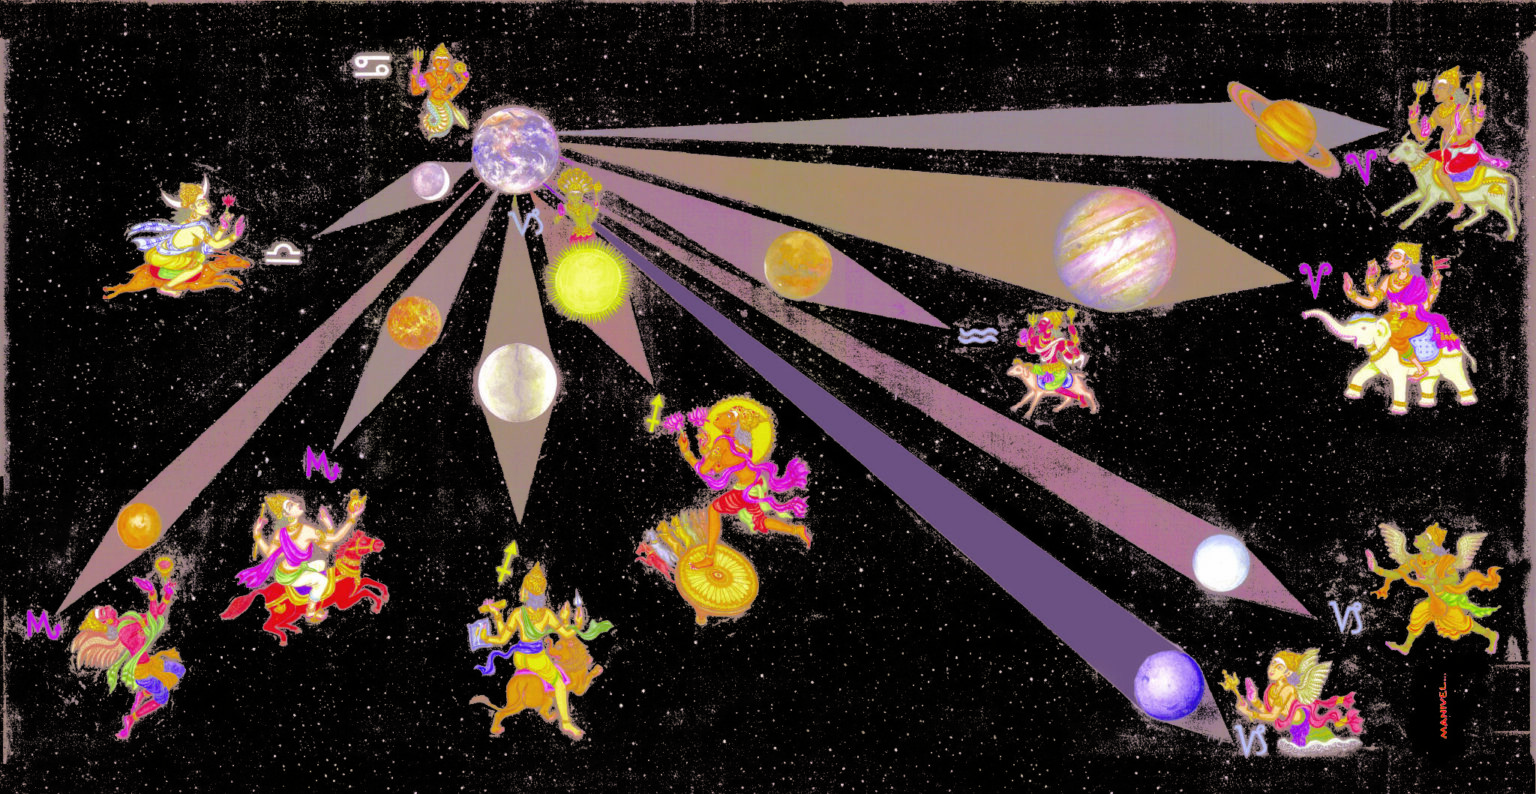
\includegraphics[width=0.8\textwidth]{pics/intro1.png}
\caption{Jyotish}
 \end{figure}

\subsection{BOOKS AND CDS FOR COURSE}
 

Astrology of the Seers: A Comprehensive Guide to Vedic/Hindu Astrology is the main book required for the course,
With Ayurvedic Astrology: Self Healing through the Stars for Part II is also required for the course.
Jyotir Bhava, Vedic astrology Mantra CD of Yogini Shambhavi Chopra (Lotus Press). This is recommended for all students wanting to know the correct pronunciation of the main mantras to the planets. Links to these chants can be found in the course and on the website.
      We generally recommend that the student complete this course material before embarking on an extensive study of traditional Hindu astrological literature, but this is left up to the discretion of the student. Traditional Hindu astrological literature can be cumbersome and without the proper background it is difficult to approach.  However, once the student has grasped the basics of the system, a study of such classics as the Brihat Parashara Hora Shastra, Brihat Samhita and Brihat Jataka (of Varaha Mihira) can be very helpful.  

\subsection{VEDIC SOFTWARE}   Many good software programs in Vedic Astrology exist notably Parashara’s Light. We recommend that the student purchase a good software programs in order to run and study charts on their own. Most software programs provide demos for you to explore and see how they work. The calculations required for Vedic charts is extremely difficult and time-consuming otherwise. There are also now some very inexpensive but more limited programs like Jyotish-D for iPhone and IPad. Note that we do not represent, nor do we receive any payment for any student who orders any Vedic software.


\begin{figure}[H]
 \centering
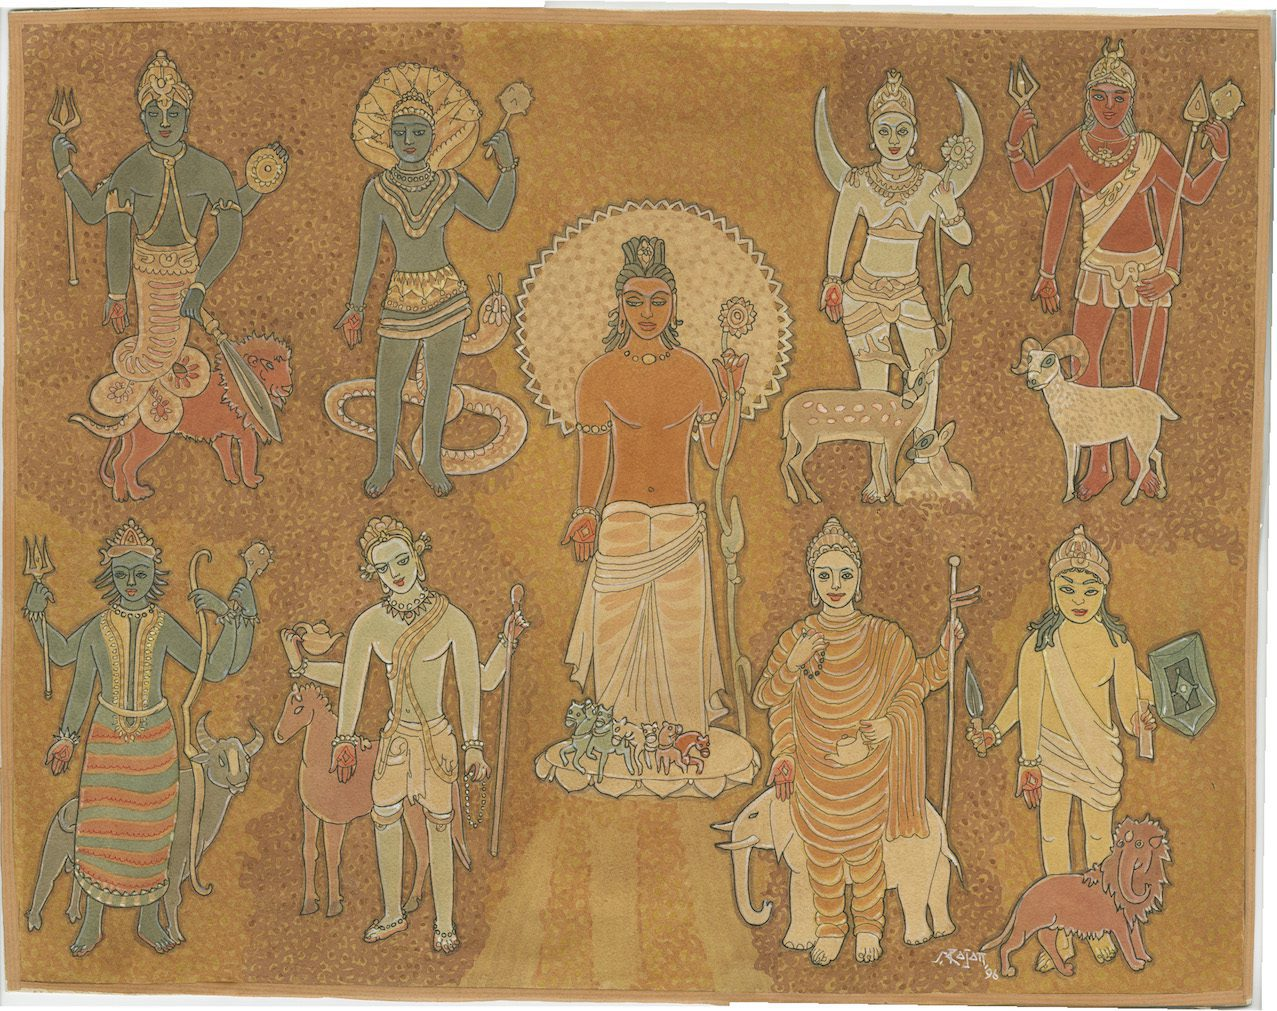
\includegraphics[width=0.8\textwidth]{pics/intro2.png}\caption{Planetary Deities}
 \end{figure}


\subsection{FORMAT OF THE COURSE}
  The course consists of 4 parts:

Part I deals with the main interpretative factors of Vedic Astrology, the foundational material.
Part II deals with Ayurveda, factors of Medical Astrology and remedial measures in Vedic Astrology.
Part III gives specialized, advanced and supplementary material on topics such as Nakshatras, Horary Astrology and Ashtakavarga.
The Workbook stands as a fourth section and is used along with the other booklets starting with Part I, will be noted in the course material.
 
\subsection{Course Workbook}
The Workbook is intended for usage in the following way:

Lessons 1-4 of the Workbook should be examined along with Part I of the course. There will be indications in Part I and at its end about this.
Lessons 5-7 of the Workbook should be examined along with Part II of the course. There will be indications in Part II and at its end about this.
You can examine the appendices in the Workbook at any time as these are for general reference.
  The Workbook is meant to provide technical and practical material, including example charts. It contains study exercises but no questions. However, a few of the questions in the tests at the end of Part I and Part II are based upon the Workbook and cannot be answered without completing it. The Workbook is particularly important for those seeking advanced training in Vedic Astrology. Others may find the Workbook to be challenging. They should be patient and realize that such application is necessary in order to learn to read charts.  

\subsection{COURSE ILLUSTRATIONS}
Course illustrations derive mainly from the Hinduism Today magazine and monastery and are under copyright. Please honor this.   COURSE AUDIOS AND VIDEOS Courses contains numerous audios and several videos to enhance the course material. These are being added to over time.  


 

\subsection{Final Test Questions}
At the end of each of the three main sections are certain Final Test Questions. The student should complete these test questions and send them to the Institute for grading.
Only if these three final tests are answered will the student receive certification for the course.
Course progression percentages are merely book marks of where in the course you have opened to the lessons. These percentages do not indicate actual course completion, which is only indicated by completion of final tests.
You can copy the tests from the on-line course material and add your answers and then send to us by email at vedicinstitute@gmail.com.
Send tests back in Word or Pages attachment. Do not send in PDF or embed in your email. This makes it easier to keep track of your tests.
Please include your name, the date you signed up for the course and your address on the test.
As it is an open book test we expect the student to answer all questions correctly.
You can also ask whatever additional questions about the course material you have along with the tests.
It usually takes us a day or two and up to a week to answer final tests. If you have not heard from us after that, please resend your tests, as sometimes tests do get lost in the spam mail.
 

\subsection{\textbf{SPECIAL AUDIO INTRODUCTION TO THE COURSE BY DR. DAVID FRAWLEY (VAMADEVA SHASTRI)}}
    

\subsection{VEDIC ASTROLOGY READINGS FOR COURSE STUDENTS}
Consultations
Those looking for Vedic astrology consultations can schedule these with Yogini Shambhavi Chopra, Shambhavi.yogini@gmail.com. Shambhavi provides an excellent approach to Vedic counseling through Vedic astrology. For students wishing to have Vedic astrological readings with us, you can arrange a reading with Yogini Shambhavi Devi (shambhavi.yogini@gmail.com), who is our resident Jyotishacharya. Yogini Shambhavi is one of the most respected women Vedic astrologers and Yoga teachers in India and the West.        Such readings can be very helpful in understanding Vedic astrology, as well as how to give readings, but are not included in the course and have their own separate charges.  

\subsection{OUR WEBSITE AND SOCIAL MEDIA}
 

Our web site at WWW.VEDANET.COM contains many articles, publications and resources.
  It includes a listing of books on Ayurveda and other Vedic topics by Dr. Frawley, and a set of over one hundred articles by Dr. Frawley on various aspects of Vedic knowledge, including sections on Ayurveda, Yoga and Vedic astrology. It contains extensive information on Yogini Shambhavi Devi, including her teachings and astrological consultations. Our various programs, intensives and travels are explained in detail. We advise the student to look at these website resources periodically for additional information in the field.  

\subsection{OUR FACEBOOK ACCOUNT FOR AMERICAN INSTITUTE OF VEDIC STUDIES} – for articles, retreats, travels and programs relative to the institute – https://www.facebook.com/americanvedic/
Dr. Frawley’s FACEBOOK ACCOUNT at https://www.facebook.com/drdavidfrawley – Regular information about Dr. Frawley and his many articles, programs and activities in the greater Vedic field, including his work in India, with over a hundred thousand followers. Not specific to Vedic astrology.
Yogini Shambhavi’s FACEBOOK ACCOUNT at https://www.facebook.com/yogini.shambhavi/ – Yogini Shambhavi’s special teachings, information and resources on Shakti Sadhana, Women’s Healing and our Yoga and Ayurveda retreats.
 Dr. Frawley’s TWITTER ACCOUNT at https://twitter.com/davidfrawleyved –  Features Dr. Frawley’s educational and social work in India, with six hundred thousand followers, which includes noted leaders, writers and spiritual teachers. Not specific to Vedic Astrology.
 

\subsection{COURSE REFUNDS AND TERM FOR COMPLETION} For such on-line courses, refund must be requested within thirty days. There will be a $50.00 processing fee taken out of the payment for our time involved. You have up to three years to access and finish the course.  

\subsection{CERTIFICATION}
  Certification for the course is given through THE AMERICAN INSTITUTE OF VEDIC STUDIES. The course provides certification for 300 hours of study in Vedic Astrology (which is how long the course, its exercises and tests, and books should take to complete), and the title AYURVEDIC ASTROLOGER: FOUNDATION COURSE.   As our institute has its own global recognition, this certification has value in its own right, particularly for combining Ayurveda with Vedic Astrology. You can also call yourself a student of Dr. Frawley, who is one of the most respected Vedic teachers in the world today.   Certification in this distance learning course does not mean that you are a fully qualified Vedic Astrologer but that you have a good foundation of information in which to become one. The course is a first stage in training in Vedic Astrology, which usually takes two years in order to become competent in the subject, like any technical discipline or profession. Yet it provides you much useful information to use for the rest of your life.  

\subsection{FURTHER TRAINING OPTIONS WITH US} Additional Programs

This course goes along with our other online courses, Ayurvedic Healing for those who wish to study Ayurveda more deeply, Integral Vedic Counseling for those interested that topic, and Yoga, Ayurveda, Mantra and Meditation for those who wish to integrate the spiritual and psychological aspects of Yoga and Ayurveda.
Dr. Frawley does take on a few students for special advanced training with him personally.
Integral Vedic Master Educator Certification, Ayurveda, Raja Yoga, Vedic Astrology, Vedic Counseling. For select students who have completed all our four courses and want a background recognition of the interconnection of their studies.
For advanced study you may consider more in-depth programs on any of the Vedic Sciences, if you have not studied these, including Yoga, Ayurveda, Vedic Astrology and Vastu. Note our courses in these fields. You might also want to take consultations with various practitioners in these fields. Dr. Frawley takes on a few private students. You can contact us if you are interested in this option. Generally this is limited to those who already have studied, practiced or taught the Vedic teachings for a number of years. It usually requires that you attend some of our retreats as well

Dr. Frawley is available for special Vedic Counseling Sessions that can also help guide you in your Vedic Counseling Practice.
 

May your study and practice of Vedic Astrology prove fruitful, transformative and enlightening! Sri Veda Purushaya Namah! Dr. David Frawley (Pandit Vamadeva Shastri)  

Namaste! 

\subsection{INDIAN NATIONAL TELEVISION (DOOR DARSHAN) INTERVIEW WITH DR. DAVID FRAWLEY}
The link is to aninterview of Dr. Frawley that explores his approach to Vedic knowledge, including Vedic astrology. For those of you who are not familiar with the scope of his work, please view it. It will help you understand the spiritual and philosophical background for this course. With Rajiv Mehrotra, not film maker and associate of the Dalai Lama. You can view it directly here. \url{https://www.youtube.com/watch?v=O0uxv-KBQgA}


\newpage

\section{THE BACKGROUND OF VEDIC ASTROLOGY}
 

The following lesson introduces the student to the background issues of Vedic Astrology and the Vedic way of approaching astrology, applying it, and what the karmas involved may be, both for the client and the astrologer.

 

\subsection{SYSTEMS OF ASTROLOGY – EAST AND WEST}
 

Vedic Astrology is a “sidereal” astrology. This means that it uses the sidereal zodiac or the zodiac of the fixed stars. In this regard, it differs from most Western Astrology, which employs the “tropical zodiac” or the zodiac of the equinoxes. The two zodiacs are currently around 24 degrees apart according to the Ayanamsha used, with the Vedic sidereal zodiac falling behind the tropical zodiac.

 

To put it simply the tropical zodiac always begins the zodiac with the point of the vernal or spring equinox as representing the beginning of the sign Aries. The sidereal zodiac calculated the beginning of the sign Aries from a  certain point in the fixed stars. As the point of the equinox is moving backwards in the zodiac over time, the different between these two systems is now considerable and the calculations of planetary positions relative to them will vary by nearly one sign. While the sidereal zodiac of the fixed stars that Vedic astrology used can be viewed against the actual constellations in the sky, the tropical zodiac is a mathematical abstraction that cannot be seen in the sky as its boundaries are changing over time.

 

In general terms, we refer to Vedic astrology as sidereal and western astrology as tropical as these are the dominant systems. There is, however, a “Western Sidereal Astrology” introduced in the early twentieth century, which uses the sidereal zodiac but otherwise follows the aspects, house orientation and other methods of Western Tropical astrology. This is the basis of the “Fagan-Bradley” system. It arose through the influence of Vedic Sidereal astrolo­gy, but also argues that the original Western Astrology was a sidereal system. We may, therefore, call Vedic Astrology “Eastern Sidereal Astrology” but as Vedic Astrology is a simpler term.

 

There are also a few Vedic astrologers who use Vedic principles relative to the tropical zodiac, or who even claim that the original Vedic zodiac was tropical, but their numbers are very few, and they are not endorsed by the majority astrological community in India.  We find that view to be unfounded and misleading as Vedic texts for thousands of years have pointed out the shifting positions of the equinox and solstice points relative to the fixed stars.

 

In any case, different systems of astrology like different systems of healing are possible, and their principles can be different. Here we are aiming at classical Vedic astrology such as has dominated in India for many centuries and is sidereally based. We are not saying other systems may not have their value. However, there is only one zodiac and we find dividing it according to the fixed stars makes more sense as a way of understanding stellar influences, than dividing it by the equinoxes.

 



 

 

\subsection{THE ASTROLOGER AS LIFE-COUNSELOR}
 

The astrologer functions as a “life-counselor,” able to address all domains of life, including health, psychology, career, relation­ship, and spiritual issues. The field of astrology is the field of life itself. There is probably no other field that has such a broad scope of applications. The astrologer can specialize in one area but needs to know something of the whole of life. Astrol­ogy shows us the basic energetics of our lives in all their different dimensions. Some astrologers may take more limited roles or simply aim at providing information, not advice. But we feel that the life-counselor model is more useful and a better basis for practice, particularly in the West.

 

To be an astrologer, therefore, can be a more holistic career than to be a  psychologist or therapist of any kind. It requires a breadth of view and capacity to contemplate life as a whole. It may be the ultimate holistic occupation. To really do Vedic Astrology requires an integral approach and pyramidal vision, such as is revealed in the system of Vedic Science that covers all aspects of life. The astrologer should guide his or her client through the domains of life toward the full unfoldment of the soul, not through giving rigid directions or predictions but through pointing out the full scope of the clients potentials along with practical tools for developing their energies properly.

 

The astrologer should therefore study Yoga, Ayurveda and related Vedic subjects in order to be competent in this comprehensive approach. It is not necessary to master all of these subjects before attempting astrological readings, but one should gradually learn their fundamentals. Some astrologers possess much knowledge intuitively. Others bring it forward from different kinds of learning that they have already done.

 

Good astrological knowledge itself may not be enough to be a good astrologer. Just because we can see how the stars affect people or when events may occur in their lives, this may not be enough to help them understand these events or use them properly. There may be those who are good astrologers in some way or another. They may have good predictive powers but they may be unable to guide anyone in the higher goals of life. This requires not only astrological knowledge but spiritual development and integrity. A Vedic Astrologer should themselves follow a spiritual discipline, practicing yoga, meditation, mantra or rituals daily, and leading a life of honesty and integrity.  Their aim should not be to seek wealth, fame or power but to be of genuine service to their clients.

 

\subsection{THREE MODELS OF VEDIC ASTROLOGY}
 

Several different models of astrology exist. Two commonly related methods in Vedic Astrology today are the “predictive” and “judgmental” systems. Some people identify Vedic Astrology with these as a rigid and deterministic system. This is a misunderstanding. Vedic Astrology is also a very important counseling system, though it does have its predictive value.

 

\subsubsection{1. PREDICTIVE ASTROLOGY}
 

Predictive astrology aims at predicting specific events in life. These are mainly mundane events such as the timing of marriage, birth of children, the time of death, onset of various diseases, accidents, financial gains or losses, times of good or bad fortune, even the times of renunciation or liberation on a spiritual level.

 

The predictive astrologer aims at being able to predict events as specifically as possible. To this end, he may use not only the birthchart but also divisional and horary charts. These predictions may extend into the world at large, predicting wars, earthquakes, election outcomes, economic trends, stock market activity and even the weather, which are all part of mundane astrology.

 

Predictive astrology is linked to the timing of events. It is concerned with planetary periods, progressed charts, transits, horary charts and electional astrology, where timing is most important. It studies how outer events reflect astrological patterns and predicts the timing of their fructification.

 

From the standpoint of predictive astrology, the skill of the astrologer is judged by the accuracy of his or her predictions. The astrologer becomes a kind of weatherman for astral influences in life. There is not always something spiritual about such skill, but it can be allied with deeper insight. Such knowledge does not necessarily show us how to rightly deal with these events in our lives, although it can be combined with that as well.

 

From the standpoint of Vedic Astrology, predictive ability is important in an astrologer and it is a skill that all Vedic astrologers should strive to develop. If we cannot determine the astrological influences behind the events of a person’s life, we may not be able to determine how they affect them at a deeper level. Such outer events allow us to verify the chart and reflect the accuracy of our chart interpretations. This does not mean that we must always be able to tell our clients when specific things will occur to them on a daily basis but that at least we should be able to show them the major trends of their lives. Actually predicting specific events in the future is very difficult and has its dangers as we may be interfering with a person’s own power of judgment.

 

The predictive side of Vedic Astrology is probably the best of any astrological system and affords it much value. Many people approach it for this alone, particularly people from India who have a more uncertain material life. But it should be used to help clients put the events of their lives in proper perspective, integrating it into a spiritual approach that shows them how to use these events for spiritual development. It should not degenerate in giving the person the view that their life is mapped out or that they are victims of fate. In addition, until one has spent many hours examining a person’s chart and subchart it is not possible to understand the short term trends and indications in the chart. A mere general life-reading cannot do this.

 

 

\subsubsection{2. JUDGMENTAL ASTROLOGY}
 

This form of astrology aims at judging the different aspects of the life and character of a person: Their health, longevity, career, finances, marital happiness, level of intelligence, stage of spiritual evolution, and so on. It is similar to the predictive method, but looks to general capacities rather than to specific events. Most importantly, it has an ethical or spiritual side that some people are sensitive about. Many people do not like to think that they can be judged from a chart or that there is any limitation to their fate or destiny. However, Vedic Astrology, with its karmic orientation, acknowledges the history of the soul and the opportunities and limitations of each person and integrates this insight into its system.

 

Judgmental astrology places a value judgment on astrological positions. Some aspects are said to be good or bad, some planetary combinations are said to make a person good or evil, or intelligent or stupid. It often has an implied moralism that we should be very careful about, as karma is full of mystery and different indications.

 

Astrology should be capable of providing helpful judgments in life. But these should not be simplistic or subjective. They should be based upon spiritual goals and should not exalt worldly success or outward happiness as being of ultimate value. For example, a chart may indicate disease. This, however, is not necessarily something bad. It does not necessarily mean that person did something evil in their last life for which they have to pay. Disease can be an important means of awakening the soul. Therefore judgments in astrology should be applied with discretion. While astrologically we can see trends and tendencies, we should never deny the freedom of the soul to awaken and transcend its karma inwardly, even when it cannot change it outwardly.

 

Both the Predictive and the Judgmental models of astrology can have a fatalistic note about them that inhibits taking control of our own lives. Predictive astrology tells what is going to happen to us, as if we had no free will in life. Judgmental astrology tells what our nature is, as if nothing could be done about it. If we apply them in too matter of fact a way, we will encourage a fatalistic attitude in our clients. They will take their good fortune or misfortune too seriously, with finality, and lose the capacity for creative and spiritual growth in life. They may feel insulted or degraded by negative judgments and predictions, or flattered by the positive ones. Neither response leads to right action in life.

 

This fatalism occurred in medieval Western Astrology that also was judgmental in nature.  It was linked to a culture that believed in the predestination of the soul, and in an eternal heaven and hell. Such fatalism cannot exist in the Vedic system which is based on karma. Karma is not fate or predestination. It is a law of cause and effect in which our present state is the result of our past actions. We create our own destiny but we do so through time, in which who we are today has already been shaped by what we did yesterday.

 

Vedic Astrology does recognize the limitations of past karma, which can be very difficult to overcome, but it also teaches us that we can change our future. The future is the result of present actions, just as the present is the result of past actions. Vedic Astrology therefore encourages individual effort, not passivity, which is why remedial measures are so important. That past actions have influenced our present state does not mean that we should just accept our condition as limited. It means that we should act in a way today so as to ensure a better future and a more positive forward movement of our karma.

 

This course does not limit itself to Predictive or Judgmental methods, though they are used within it. The Predictive method, if applied superficially, becomes too mundane in nature. It can turn the astrologer into a mere fortune-teller. It gives people the impression that their destiny in life is fixed and that a good astrologer can remove any mystery about what will happen to them.

 

We should add that prediction is easier in a fixed and traditional culture like India. In the modern West, many of these predictive rules fail. For example, the potential for divorce is much higher in western culture today. For this reason, the traditional Hindu rules of marriage do not always work on charts of people in the West. Hence, these rules must be altered. They can show ease or difficulty in relationship, but how that translates into marriage or divorce is conditioned by the time and by the culture.

 

The Judgmental method can be too harsh. It can deprive people of the capacity for growth. It can reinforce any negativity in the chart. Even if the outer chart has many weaknesses, it should never be forgotten that our inner Self and true Being inherently transcends the influences of time and space. This method is particularly dangerous with passive, self-negative types of people who easily believe what is told to them, and are ready to accept something negative about themselves. It often becomes a self-fulfilling prophecy.

 

Personally, I think there is undesirable karma in following these methods too strongly or rigidly. To tell a gullible person that they have certain limitations in life or that they will suffer some difficulty at a certain time may make it occur. The astrologer should act in such a way as not to deprive the client of his or her own power of judgment. The astrologer can give clients information or tools to work with but they must not take power over their clients. The astrologer is not God and the birthchart is seldom so fixed that all astrologers will interpret it in the same way. Therefore, the astrologer should not be too proud or convinced of his or her opinions. He should remain open to the fluidity of life. While we may have to warn our clients of the effects of wrong actions, this should stimulate them to a better way of living, not make them feel that they cannot change their condition.

 

There is yet another approach to Vedic Astrology that we should note. This is more the flattery method in which the astrologer tells the client everything good about them and their chart. It may be done in an effort to show people the positive side of their nature or it may just be done to gain more clients. If we do not point out the difficulties inherent in a chart, we are also doing our client a disservice. We should point these out in a way that enables the client to use them as a basis for greater growth and understanding. We should neither ignore them nor present them in a rigid manner. We should point out both the positive and the negative objectively and try to give the client the tools to use the higher potentials in their chart – and there is seldom a chart without them.

 

\subsubsection{3. SPIRITUAL ASTROLOGY AND ASTROLOGICAL COUNSELING}
 

The system taught in this course is more a form of spiritual astrology and astrological counseling. It uses astrology as a tool for self-knowledge and an aid in Self-realization. It uses the cosmic forces transmitted to us through the planets to connect us with our own deeper cosmic nature. In this regard, I always teach my clients the basic meaning of the planets in their charts and the characteristics of their planetary type. This allows them to enter into the process of astrological knowledge which is necessary for astrology to become a useful tool for self-growth.

 

It employs predictive and judgmental methods but in a broader spiritual context. I try to acquaint my clients with both the good and bad potentials of their chart and offer them the tools to augment the good and ward off the bad. I do not leave my clients victims of fate. I teach them that their soul transcends time and that it can use the energetics of the chart in several ways. I do not recognize an absolute fate in life but only probabilities that can be high, medium or low.  For example, I may tell a client their chart is not good for relationship or that it may be prone toward divorce, but I would be hesitant to tell them that marriage is impossible (though there are cases of this). I would hesitate to give a person the date of their divorce when a difficult period for marriage is indicated. However, I would inform them if a relationship were unlikely to endure through a given planetary period.

 

This approach does not aim at prediction alone. I am more concerned with helping the client to manage their planetary energies rather than merely telling them what is likely to befall them for good or ill. I relate to them favorable or unfavorable periods for different ventures or affairs and help them guide the course of their lives through these. I encourage them to action on all levels through the remedial measures of Vedic Astrology and its related systems of Yoga and Ayurveda. I believe that the proof of a good astrologer is how he or she makes their clients aware of their astral influences and how to better manage them, not how good he or she is at predicting particular events only. Such an approach is not aimed at making the individual more tied to his external nature but opens up the potentials of the spiritual life which the individual may not yet be using or even be aware of.

 

\subsection{THE ASTROLOGY OF HEALING/ YOGIC ASTROLOGY AND AYURVEDIC ASTROLOGY}

 

Astrology requires a healing method to be really useful. We must not only be able to recognize planetary influences in our lives; we need to know how to harmonize them. We must help our clients learn how to balance the planetary influences in their lives.

 

An astrology of healing has two levels: First, Vedic astrology has measures to treat our outer nature and, second, those to treat our inner nature. The outer nature, our body, senses and conditioned mind, can be treated by medical and psychological methods that are not specifically astrological in nature. Our inner nature, our soul, requires occult and yogic methods and ultimately rests upon our own effort to grow spiritually in life. This has more scope for astrological healing measures.

 

Vedic Astrology is not just a predictive or interpretative system.  It is also a remedial system with techniques and methods for balancing planetary influences. These are as essential as the interpretative side. What use is it to tell people what is going to happen to them if we cannot give them a means of dealing with it? For this reason, the second part of this course includes such remedial measures as gems, mantras, yantras, herbs, and color therapy, and the role of Ayurveda as well as Yoga.

 


\subsection{THE FOUR AIMS OF LIFE}
 

On this foundation of examining the different models and goals for Vedic astrology we will now introduce the Vedic view of life. Vedic Science traditionally recognizes four legitimate aims or goals of human life: Dharma, Artha, Kama and Moksha.

 

DHARMA means “principle or law” and refers to the fulfill­ment of our right purpose in life.  It includes the honor or recognition we attain through our actions on a personal and professional level, specifically through the medium of career. It relates to broader principles of truth and right action. Ultimately it refers to our soul’s purpose in this incarnation.
ARTHA means “achievement of goals” and relates specifically to the acquisition of material resources required to fulfill ones dharma in life.  It relates to income and wealth.
KAMA means literally “desire” and refers to our need for emotional and sensory happiness. As such, we could call it “enjoyment.” But lasting happiness is only possible when we fulfill our dharma.
MOKSHA means “freedom” or liberation and relates to our need for spiritual growth, including transcendence of the above three lower values.
 

Vedic Astrology recognizes the validity of all four aims and is oriented to facilitate the human being in the attainment of each of them. Yet in Vedic Science the first three, career, wealth and enjoyment are subordinate to the last, spiritual liberation. Liberation is the primary and essential goal for all human beings. Without it, the other goals have no real meaning. The others are merely a support for it and have no validity in themselves. An astrologer using the Vedic system should, therefore, give a comprehensive view of all the domains of life. Yet he should focus on liberation and the spiritual life. This does not mean to take the role of a guru but to show the higher usages that can be made of the planetary energies and circumstances in ones life.

 

From the Vedic perspective, a chart that is good for liberation but not for the other domains of life is a much better chart to have than one that is good for the lesser goals but not for the spiritual life.

 

As a foundation for the four aims of life, astrology addresses the need for health, arogya, or freedom from disease. This is the basis for the four aims of life, for without health, what else can be accompli­shed? Yet health is not just physical, it is also mental. So astrology must consider physical and mental health or physical health and psychological well‑being as the means of approaching all the goals of life. Hence, medical and psychological astrology, after spiritual astrology, are its most important branches.

 

I have addressed some of the astrological indications of these factors. These will be more understandable later on in the course.

 

 

\subsubsection{DHARMA}

 

Dharma refers in a broader sense to the spiritual principles and natural laws that govern the universe. In the individual context it refers to our basic nature, inclinations and capacities in life. Dharma as career, refers to right vocation and the happiness inherent in fulfilling ones capacities for right action in life. Ones true Dharma is that of ones soul, our hearts vocation, not what society imposes upon us. Yet most of what we call Dharma is revealed by our occupation in life, how we earn our livelihood.

 

Under this concept are also included honor, position, status, fame, prestige and power. These show our social dharma and its effects, including how our character affects the world. Our individual dharma should reflect in some way the universal dharma. If our dharma is adharmic; that is, if our career is harmful to others, then it will end up harming ourselves as well.

 

Dharma is related to Artha, the objects and goals that we seek to attain things in life. Usually it is through our career that we seek wealth.

 

 

\subsubsubsection{Indications in the Chart}

 

These indications will make more sense later in the course after students are more familiar with the planets. Please remember it for future reference.

 

Jupiter, Mercury and the Sun are the main planets that rule Dharma. Mercury shows how we function and communicate in society. Jupiter shows the role or law we like to follow in life, our guiding principles and the goals we seek. The Sun shows our ability to project our character and personality, the influence of our nature on the world.

 

Dharma houses are the first, which shows our personal dharma and responsibility to self, the fifth which shows our creative dharma and responsibility to children, and the ninth that shows our spiritual and social dharma.

 

For house influences, we should note that of the first, ninth and tenth houses and their lords. The first tells us who we are generally; it is the measure of our identity and action in the world. The ninth shows the goals or profession we aspire to. The tenth measures our capacity to impact the world karmically. It shows how our personality appears in the world. It shows how our dharma achieves artha, or value, both for ourselves and for society.

 

 

\subsubsection{ARTHA}

 

Artha, wealth, refers to all necessary means of material livelihood and security, not simply the pursuit of material gain. The astrologer should be able to counsel his clients on how to best use their material potential in life. This is in directing it towards spiritual or dharmic ends, not simply pursuing money for the power or status that it may afford.

 

 

\subsubsubsection{Indications in the Chart}

 

The planets that rule Artha are Jupiter and Mercury. Jupiter governs our capacity for gains and abundance generally. Mercury rules our ability for commerce and exchange. Venus also gives wealth and comfort, art or luxury. Saturn tends to create poverty (though it can give us property and other hard or fixed assets).

 

Houses of artha are the second, sixth and tenth. The second shows how we gain our personal livelihood. The sixth shows work capacity and money from sources such as insurance or legal settlements. The tenth shows career gains, staus and achievement.

 

In particular, we should take into account the influences on the second and eleventh houses and their lords. The second governs our ability to earn through our own labor, the eleventh to gain income from various sources. After these we should consider the fourth, fifth and ninth houses and their lords, which all give wealth. The fourth gives property and vehicles. The fifth gives gain through counseling, advice and speculation, like the stock market. The ninth gives grace and fortune, like the winning of lotteries.

 

The twelfth, sixth and eighth houses and their rulers tend to limit wealth. The twelfth shows loss and expenses. This in itself may not create poverty if the houses of income are strong. The sixth gives loss through disease, enmity, legal problems, overwork or lack of recognition. The eighth shows difficulties, obstacles, oppression, lack of recognition or bad reputation.

 

 

\subsubsection{KAMA}

 

Kama, enjoyment, refers to all legitimate sensory enjoyments, not just pleasure in the gross sense but the enjoyments natural to the right use of the senses. To enjoy life, to appreciate the beauty of nature, true art and loving communication between human beings, is part of the fulfillment of our soul and need not be denied for spiritual growth. In fact, all life is a seeking of happiness. It springs from joy itself. If we were not in some way happy or able to find happiness, why would we wish continue living?

 

Our enjoy­ment or pleasure in life is largely through relationship, which includes sexuality. Hence, relationship is the main factor of Kama and its issues of love, marriage, partnership and children. The higher level of Kama or enjoyment relates to our artistic sense. The highest level relates to our capacity for devotion, our openness to Divine love, beauty and delight.

 

 

\subsubsubsection{Indications in the Chart}

 

The planet that rules Kama is Venus, the planet of desire. According to its position in the chart, our capacity for enjoyment or Kama can be read. Mars is also important as it shows our goal-seeking in life. Aligned to Venus, it often takes us along the realm of desire. Jupiter gives us capacity for enjoyment or happiness of a more general nature, while Saturn tends to deny or limit it. Saturn aligned with Mars may cause us to seek perverted or unwholesome means of enjoyment.

 

Kama houses are three, seven and eleven. The third is the house of talents, hobbies, curiosities, interests and sports – personal kama. The seventh house is the house of love, marriage and fulfillment in human relationship – relationship kama. The eleventh is the house of friendship, expression, social and career gains – social kama. The fifth is also important as the house of romance, joy and creativity, the happiness that comes from dharma. The twelfth is the house of secret pleasures and hidden desires and has some relevance as well and also indicates the happiness that comes from moksha.

 

 

\subsubsection{MOKSHA}

 

Moksha, liberation, refers to our work of Self‑realization in life, our efforts at Self‑knowledge. It includes whatever liberates our inner spirit and creative force in life. In its proper domain, it transcends organized religion and codified beliefs and is ultimately an individual affair.

 

The pursuit of various forms of knowledge, including philosophy, science and the occult, as well as creative expression, like art, are themselves lesser aspects of the goal of liberation. For this reason, the aim of liberation can also be defined as knowledge. All of us are seeking knowledge or freedom in one way or another. It is knowledge that gives us freedom, which extends our horizons and gives us access to the greater world beyond the limits of our body and senses. Yet knowledge may be lower, as of the outer world, or higher, as of the true Self. This latter is the real goal through which real liberation is possible. The lesser knowledge gives us greater space to operate in the world but it does not free us from the limitations of worldly existence.

 

 

\subsubsubsection{Indications in the Chart}

 

Jupiter and Ketu rule Moksha. Jupiter shows our general seeking of expansion and truth, our aspiration and need to grow and transcend. Ketu shows our ability to negate and transcend things. It affords deep insight, discrimination and perception. Saturn is also important as it gives detachment, renunciation and the capacity to be alone. Mercury is important, as the indicator of the intellect; it shows the level of knowledge that we seek.

 

Houses of Moksha are fourth, eighth and twelfth. The fourth shows our emotional happiness. The eighth shows occult and mental insight. The twelfth shows spiritual liberation.

 

The house influences of the ninth and twelfth together are important, as well as their lords, with Jupiter the significator of the ninth and Ketu of the twelfth. The ninth gives us our sense of values, goals, principles and aspirations. It shows the dharma behind our pursuit of moksha. The twelfth allows us to negate our experiences and go beyond what we already are (our conditioned being). It also shows the past and the latent impressions in the subconscious that motivates us. The fifth house has some importance as the measure of the good karma we bring into the present life, the indication of past spiritual practices. It also shows our devotion in life, what form or energy of the Divine that we seek.

 

The fourth and eighth houses also relate to liberation. The fourth shows our capacity for peace of mind, the foundation of all spiritual pursuits. It shows self-contentment, psychological stability and mental receptivity. The eighth shows our ability to go beyond death and time, the gateway to the eternal. It gives the ability to transcend suffering and often affords deep perception.

 

The planets of ignorance and attachment often limit our pursuit of Moksha. These are particularly Venus and Mars, the planets of passion and sexuality. Saturn can provide the detachment that aids us in liberation or it can create darkness of mind that prevents it. Jupiter can get us attached to outer affluence or religious ceremonialism. Hence, liberation is the most complex thing to measure in a chart. All planets have a higher or spiritual and lower or materialistic functioning.

 

Jupiter, as the great benefic, is the planetary indicator of our positive goals in life. So it is the most important planet in showing how we can achieve any of the four aims of life. How our Jupiter is oriented will show the areas in which we will seek our highest good in life.

 

Saturn, as the indicator of karma or destiny, shows the limitations we encounter but is also useful in giving us the lesson of suffer­ing that takes us from the lower to the higher goals.

 

When both Jupiter and Saturn balance each other and further spiritual knowledge, we are able to attain our maximum destiny in life and become a person of true greatness.

 

The lunar nodes have a similar importance. Rahu, the north node, shows where we are apt to overly project ourselves into the outer world. Ketu, the south node, indicates where we are prone to overly contract ourselves into the inner world. When the lords of both nodes are in harmony our lives function well. When they are in harmony on a spiritual level, great transformation is possible.

 

\subsubsection{Relationship between the Four Aims of Life}

 

These four aims are like a pyramid with liberation at the top. Each is meant to aid in the others. We need to be happy generally in order to function at all. We need the resources to enable us to have leisure and peace of mind. We need the acknowledgment or recognition of others. In this regard, a failure or inability to achieve the lower goals can inhibit the higher. If we are impoverished, degraded, ill or stupid, it is difficult to get beyond the outer aspects of life.

 

Yet most of us are caught in the lower goals and do not appreciate the higher in our true nature. Often our pursuit of the higher remains a pursuit of the lower in disguise. In the name of God, we still seek pleasure, power or fame. Astrology is also usually denigrated in such a way when its lower rather than higher insights are implemented.

 

It is important not to deny the pursuit of any of these aims for anyone but to show how they relate properly to and direct us toward the true goal of spiritual liberation. We should never encourage a client to pursue these outer goals as the highest pursuit in life. There may be times in life when it is necessary to focus on them or take advantage of the favorableness of the time to achieve them, but this can be done with a long-term spiritual orientation. For this reason, we should not give the lower goals too much weight in reading a chart. A purely business astrology, for example, would not be in harmony with the Vedic approach unless the business was oriented towards spiritual goals.

 

When we define success or failure, difficulty or ease for people based upon their charts, we must indicate in which domain and on what level. We may judge a chart as good for wealth or career, but this does not mean it is good for health or spirituality. In this way, many charts that are difficult for ordinary goals have higher blessings.

 

\subsubsection{THE KARMA OF AN ASTROLOGER}

 

The modern world does not believe in karma, but in money and the fame that the world gives us. There is the tendency to think that if our work gives us wealth and recognition then it is good. This, however, may not be the case. As wealth and recognition are outer values, they can come to us according to an outer or unspiritual orientation in life. Astrology can give wealth and fame but also deeper knowledge. The two are neither inclusive or exclusive of each other but the latter is the real grace of astrology through which alone true happiness will come to us.

 

To do Vedic Astrology properly, we must teach our clients the laws of karma and live according to them ourselves as well. Vedic astrology is the ultimate system of karmic management, both for ourselves and others. It is not our name and wealth that we take with us when we die but our karma. It is our main purpose in life to reduce our karmic burden and aid others in doing so. This is also the true role of the astrologer. A worldly astrology that flatters people, that encourages them to seek happiness in the outer world, that glorifies wealth, fame and talent, breeds more karma for the astrologer and their clients.

 

As astrology is an intimate form of counseling and deals with the deepest issues of life, it carries great responsibility. It has a power that can work against us if we apply it in the wrong manner. If we give our clients wrong advice or project them in a direction that may not be helpful to their soul, then it will be our karma to similarly be misdirected by others or to misdirect ourselves. Even if a chart is very good for outer things like wealth, we should not simply glorify such good fortune for our client but show its limitations. Similarly, if a chart is not good for the outer goals of life, we should point the positive value of such a chart for bringing us into the spiritual life.

 


\subsection{\textbf{Talk by Dr. David Frawley on Vedic Astrology and Vedic Counseling
Shows how we view and apply Vedic astrology in our integral approach to Vedic knowledge}}

\begin{figure}[H]
 \centering
\includegraphics[width=0.8\textwidth]{pics/overview1.png}
 \end{figure}

\begin{figure}[H]
 \centering
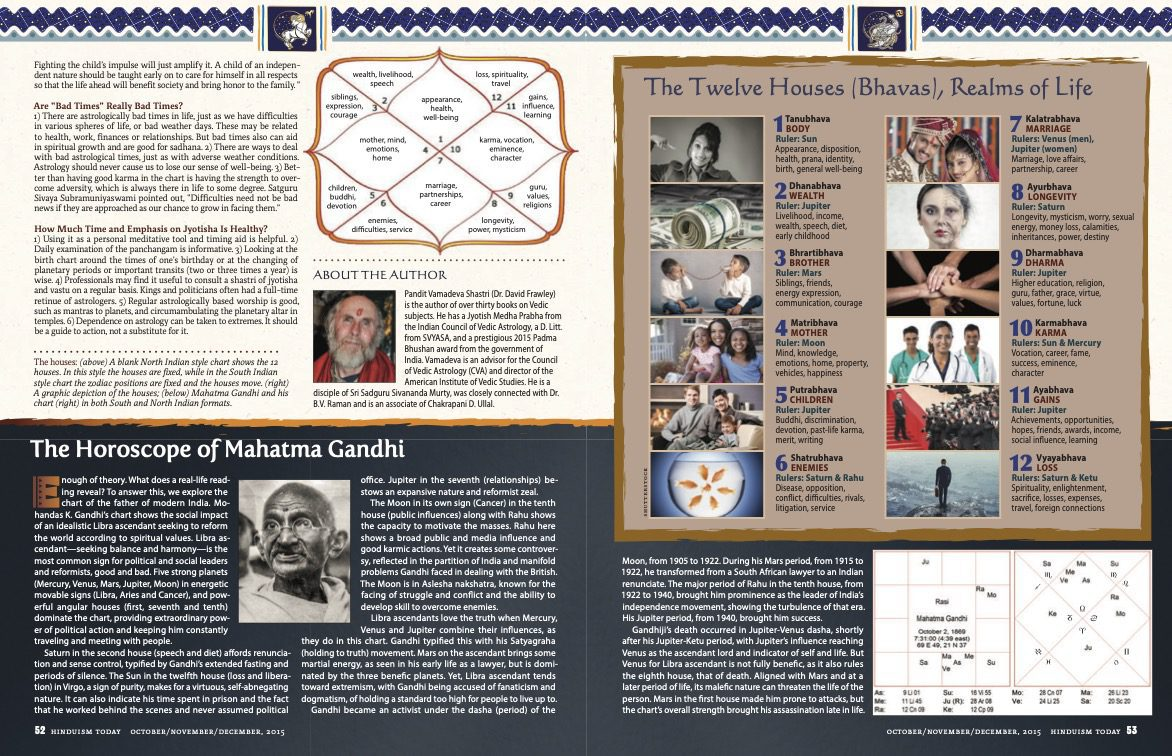
\includegraphics[width=0.8\textwidth]{pics/overview2.png}
 \end{figure}


\newpage

\section{OVERVIEW OF VEDIC ASTROLOGY}
 

This lesson is based upon a special feature issue on Hindu/Vedic astrology that Vamadeva did for the magazine Hinduism Today some years ago. It addresses the practical questions about Vedic/Hindu astrology and its applications. It does not deal with the technicalities of reading a chart that we will examine later in the course. It addresses the background, role and usage of Vedic astrology overall, and how to explain its relevance to a general audience and their concerns about its nature, validity and usage. We have recently edited and updated this lesson.

 



\subsection{EDUCATIONAL INSIGHT}
Jyotisha, Hindu/Vedic Astrology

How the Science of Light Can Help You in Daily Life

By Pandit Vamadeva Shastri

 

In the Hindu view, the planets are not mere celestial bodies circling the Sun. They are also divine beings. Each is like a prism, conveying subtle energy from the far galaxies, thus impacting man’s affairs on Earth according to its unique nature and location in the sky. The ancient science of space and time that understands and maps this influence is called jyotisha (literally “science of light”) or Hindu astrology. 

 

It’s About Time

\subsection{AN INTRODUCTION BY HINDUISM TODAY}

Believing nothing, the skeptic is blind; believing everything, the naif is lame. Somewhere between the two lies the lauded land of viveka, discrimination, which neither doubts every inexplicable phenomenon nor swallows every unexamined statement. In this issue we explore the uncanny Vedic technology of jyotisha, that hoary knowledge, derived from secondary Vedic texts, which embraces both astronomy and astrology. It’s about time.

 

President Ronald Reagan confounded the White House staff and embarrassed aides by having his itinerary and major meetings scheduled in consultation with his wife’s astrologer in California. Scoffing staffers counted it pure silliness; others thought it merely impolitic of him, maybe because of the implication that he wasn’t totally in charge or that a Christian would so publicly propound such things.

 

Mr. Reagan is not a lone heretic. Queen Elizabeth I, a Virgo, consulted the stars. Galileo, the Italian mathematician and astronomer, cast charts on the side, as did the German celestial scientist Johannes Kepler. Britain’s Princess Diane followed the stars, and many Hollywood stars do the same. Ditto with Carl Jung and American millionaire J.P. Morgan. A 2013 Harris Poll concluded that 29 percent of Americans (and nearly half of 18- to 24-year-olds) believe in or follow astrology. By contrast, 92 percent of the Chinese public think horoscopes are nonsense.

 

Like so many other things, astrology in the West is about personal things—about me and mine, my spiritual progress, my love life and business success. These concerns are not absent in the East, but larger concerns dominate. Astrology in India is about auspiciousness, about connections, about sacred timing and being in a flow with the ebb and tide of divine forces.

 

Astrology is a part of Vedic self-understanding. We look to the stars to see ourselves better, to discover the mysteries that lie all about us and within us. In rita dharma, that heavenly cosmic orderliness, stars are more than massive conglomerates of molecules or fiery furnaces fleeting afar. They are entities, potent presences that affect us despite their distance. There are, of course, many Hindus today who pooh-pooh such notions. “Stuff and nonsense,” they will cry, “What thoughtful person can accept that stars, so remote, influence life on Earth?”

 

But what thoughtful person, asks the astrologer, would deny the powerful tides dragged across our planet by a faraway moon, or gainsay the not-so-subtle solar forces that are the very stuff of life here? “Ah, but go out another few thousand light years and tell us what petty influences persist,” our doubter might challenge. The jyotishi (Vedic astrologer), realizing the basic East/West difference in world views, attempts to help the skeptic understand the Hindu perspective. “In Eastern thought, particularly Hinduism, we conceive of all existence—including the stars and planets—not as being ‘out there,’ but rather ‘in here’—within the consciousness of each one of us. In other words, consciousness encompasses all of creation. The ‘outside’ and ‘inside’ are mirror images, and the essential nature of the cosmos is not that of multitudinous distinctions but rather the many-faceted expression of a one unified Reality. Thus we do not follow the mechanistic, externalized approach typical of Western thought.”

 

The astrologer is something of a tribal shaman. Ideally, he or she is the one among us with special insight, with a wider vision that lifts awareness beyond our little world, connecting us to the canopy above, expanding perception beyond the narrow sliver of time in which we live by bringing past lives and actions into the now. You could say that astrologers tell time with a bigger watch.

 

The genuine astrologer is, in a sense, a time navigator. He teaches that time is not all colorless and neutral, the same in all directions. Time has its eddies, its waxing and waning, its preferential ways—and in that sense is much like the oceans. No ship’s captain worth his hardtack would consider the sea a uniform body of water, everywhere equal and indifferent to his passage. No, the sea is alive with idle doldrums and treacherous tempests, and, yes, dangers worthy of anticipation.

 

To the astrologer, time is like that sea, with moods and forces, some propelling us swiftly forward, others opposing our well-plotted progress. How foolhardy the seaman who keeps his canvas unfurled in a storm or stows his sails when the good winds blow. Time is a kind of moral wind, blowing now this way, now that. As a ship’s captain heeds the chart reckoned by his navigator as to course, winds and tides, so our life’s journey benefits from periodically examining another chart, our astrologer’s appraisal of protean time’s patterned flow.

 

Those who still doubt are members of a hoary club. Yogaswami of Jaffna had the perfect prescription for them, one that sets aside all of the good versus bad, will versus fate: “All times are auspicious for the pure Siva bhakta.”

 

\subsection{Working with Our Karmic Code}

Philosophically, Hindu astrology reflects the law of karma, which includes both free will and an aspect of predetermination, or fate. Predetermination means our present condition is the result of our past actions from previous lives; free will means we shape our future by our present actions—how we respond to the challenges. The birth chart represents a person’s karmic code, the samskaras with which he or she is born, imprinted on the subtle or astral body. This code is analogous to the genetic code that outlines the main potentials of the physical body. The birth chart indicates the main potentials of our entire life.

 

From an astrologer’s point of view, the birth chart is the most important document we have in life. Yet, like the genetic code, it is written in a mathematical language that requires decoding by a trained expert, and it calls for careful examination over time to unfold its dynamic secrets. K.N. Rao observed, “A horoscope reflects the allotment of karmas of previous lives. We are all getting the results of our karma, but not all of our karma.”

 

According to the Vedas, when a soul takes birth, it descends through the heavens and the atmosphere before reaching Earth, taking on heavier sheaths of material density. It can only take birth in the physical plane at a time karmically in accord with its nature and destiny. The birth chart represents the seed pattern of its life; how it develops depends upon environment as well.

 

Satguru Sivaya Subramuniyaswami advised: “When unfavorable times arise which have to be lived through (as they all too frequently do), we do not carp or cringe, but look at these as most excellent periods for meditation and sadhana rather than worldly activities. Just the reverse for the positive periods. Spiritual progress can be made during both periods. Both negative and positive times are, in fact, positive when used wisely. A competent jyotisha shastri (Vedic astrologer) is of help in forecasting the future as to when times will come along when advancements can be made. A positive mental attitude should be held during all the ups and downs that are predicated to happen. Be as the traveler in a 747 jet, flying high over the cities, rather than a pedestrian wandering the streets below.”

 

\subsection{Cosmic Consciousness}

Astrology is the science of fathoming the influence of the sun, moon, planets and stars upon living creatures. In Sanskrit it is called jyotisha, which means the “science of light”—specifically, “Vedanga Jyotisha,” the astrological limb of the Vedas, said to be the very eye of the Vedas.

 

Jyotisha is a system of understanding how our lives and our karmas relate to the movements of the cosmos, which is cognized as a single greater organism. Under jyotisha is included astronomy, meteorology and forms of divination, including palmistry, the reading of omens, svara (reading the breath) and various oracles.

 

Like yoga, jyotisha is a super science that links us with the cosmic intelligence behind nature. Its first message is that we are one with the Universal Being. New discoveries in quantum physics demonstrate the interrelatedness of the universe, showing subtle levels of immediate interaction even at great distances of time and space. Jyotisha is an integral aspect of the traditional Vedic sciences, along with ayurveda, vastu and yoga, all of which are usually used together.

 

How can the stars and planets influence events on Earth? Obviously the Sun is the basis of all life. According to the Vedas, it also projects a force of intelligence and spirituality. The Moon is important to all creatures and governs the fertility cycles of animals. In the Vedic system it rules the emotional nature. It is well known that the large magnetic and gravitational fields of the planets affect the Earth physically. That they would have subtler influences as well is not illogical.

 

Astrology is common in one form or another in all cultures, though in India it has had the widest and freest development, from the most ancient period to the present day. Ancient Greece and Rome used astrology extensively, as did Europe to the eighteenth century, even though it was often banned by the church. We could say that the type of astrology used by a culture reflects its understanding of the universe, particularly the subtle and spiritual influences guiding our lives. Curiously, modern cultures continue to employ astrology even when its validity is questioned by the scientific community. The ever-popular sun signs in newspapers reveal this undying interest.

 

Jyotisha remains an important facet of Hindu spiritual, religious and social practice, not only in India but worldwide, throughout the Hindu diaspora. It is widely used by Hindus, from common villagers to the sophisticated urban elite. It is an important component of temple worship, pilgrimages and yoga practices. It is avidly used for guiding family life, business and career, physical health and psychological well being. Jyotisha is famously employed by politicians to aid them in winning elections. This science of Vedic astrology is now going worldwide and followed by all those who wish to understand the movement of karma and dharma in their lives.

 

Hindus follow a special sacred yearly astrological calendar, called panchangam, for the right timing of all actions. India has many notable astrological and planetary temples, and new ones are coming up as astrology grows once more in popularity. Astrological icons are found in Hindu temples of all types. In South Indian temples, an altar of astrological Deities, called the navagrahas (“nine planets”), is placed in the corner of the central courtyard. After doing the clockwise perambulation around the Deity sanctum, devotees perform a second walk around the planetary Deities’ shrine.

 

Many yogis and sages have been astrologers or written on astrology. This includes modern figures like Sri Aurobindo, Ganapati Muni, Paramahamsa Yogananda and his guru Sri Yukteswar, Sivananda Murty, Swami Dayananda (Arsha Vidya Gurukulam) and historic figures like Madhva, Bhishma, Vashishta, Parashara, Bhrigu and others.

 

Newborns are traditionally named based on their jyotisha charts which provide optional syllables, based on the nakshatra, to begin the child’s name. Astrological concepts are pervasive in the organization of the calendar and holidays, as well as in areas of life such as the timing of marriage, opening a new business or moving into a new home. Hindu priests and teachers are routinely trained in astrology, among other Vedic disciplines. Introduced as an elective study at the university level in India in 2003, Vedic astrology manages to retain a position among the sciences in modern India. There is a movement in progress to establish a national Vedic university to teach astrology together with the study of tantra, mantra and yoga. All this despite complaints by some scientists.

 

From Kerala in the South to the Himalayas in the North, there is an astounding variety of profound astrological approaches, systems and techniques, including different ways of designing the birth chart.

 

\subsection{Remedial Measures}

Jyotisha does not leave us helpless before the onslaughts of karma. It provides practical ways of dealing with them. Sa­dhana invariably helps neutralize the effects of a “bad chart.” Ultimately, in fact, there is no such thing. A chart that does not portend worldly benefits, such as wealth or marriage, is likely to be good spiritually. “Afflictions” to home, family, marriage and money are often necessary for a person to renounce the world and devote himself to spiritual practices. Afflictions in the area of health can benefit from spiritual practices like mantra japa. While one career may not be favorable for success, another may be. Many remedial measures can help with karmic obstacles, including penance, pilgrimage, bhakti, praying for divine intervention, mantras and yantras, performing rituals, seva and charity. Planetary effects can be softened through special disciplines such as feeding crows (Saturn) or planting trees (Jupiter). Remedial measures are routinely recommended in Vedic, yogic, tantric and ayurvedic texts.

 

The main remedies are ritual and mantra. Propitiating the planets is an integral part of all Hindu rites. Many temples, particularly in the South of India, have a shrine with murtis of all nine planets (navagraha). You can worship them and even employ temple priests to perform special planetary pujas for you.

 

Each planet also has a name mantra (e.g., Om Sum Suryaya Namah for the Sun) and a set of special names, 108 or 1,008, that are chanted to propitiate it. Each planet has a Vedic verse and a Puranic verse used in its worship. Chants to the planets can be done singly or in combination (depending upon the recommendation of one’s teacher) while meditating on a yantra and an image of the Deity or related Deities. Scriptural verses to the Deities can also be recited. For example, Vaishnavas prescribe the Santana Gopala Stotra, to Krishna, for couples whose charts are unfavorable for bearing children. The Mahamrityunjaya Mantra, to Lord Siva, is used to counter the influences of Mars and Saturn.

 

Hindus commonly wear gemstones to balance negative and promote positive influences. Some but not all astrologers prescribe gemstones. Mantras and rituals are preferable but require more time on the part of the person. Each planet has a particular gemstone: ruby for the Sun, pearl for the Moon, red coral for Mars, emerald for Mercury, etc. High quality gemstones can be expensive. Less costly substitutes, though less effective, are allowed. Gemstones should be chosen with care and preferably with a good astrologer’s approval. They should be properly energized with mantras and rituals to function in the best possible manner.

 

Having said all that, sometimes it is better to try to learn from difficult karmas rather than trying to avoid or change them through remedial measures. We cannot buy off the planets or our karma merely by putting on expensive gems or paying someone else to take care of our life. Humility and devotion should be the basis of all remedial measures, along with a willingness to work on ourselves. Some things just can’t be changed or avoided.

 

\subsection{A Mystical Science}
 

How did the ancient Hindu rishis and yogis arrive at the knowledge of astrology? By the same means that all the other Vedic and yogic systems of knowledge arose, and by which they are studied today. Those methods include meditation and samadhi, starting with dharana or samyama, on the Sun, Moon, planets and stars. Another means is communion with planetary Deities, who can speak to us and disclose their nature and influences. Another is reason-based thinking in which we draw connections between phenomena at cosmic and individual levels. Finally, centuries of experience, study and communication among astrologers have helped turn intuition into science.

 

Eighteen traditional systems (siddhantas) are mentioned in Vedic astrology, some bearing the names of the greatest sages of Hinduism. Unfortunately, none of their texts has survived intact. Five of the eighteen were, however, summarized by Varaha ­Mihira—perhaps the greatest astrologer of classical India—in his Pancha Siddhan­tika, namely, Pitamaha (or Bhishma), Vashishta, Paulisha, Romaka and Surya. Of these, only the Surya Siddhanta has survived, and that in a later form. In addition, we have the work of Rishi Parashara, which has endured in expanded form as the Brihat Parashara Hora Shastra. That is the main text of Vedic astrology used today, containing all the essential features of the system. Many South Indian astrologers, however, use the Brihat Jataka and Brihat Samhita of Varaha Mihira, which are similar to Parashara’s overall indications.

 

\subsection{Antiquity}
 

Evidence indicates that jyotisha goes back to ancient times. The Kali Yuga calendar, which begins in 3100bce, is well known. Greeks in the fourth century bce wrote of an Indian calendar relative to ancient king lists with a beginning date of 6700bce (mentioned by Megasthenes in his Indika). The nakshatras (asterisms) are mentioned in the Rig Veda and other Vedic texts, with a Nakshatra Sukta noted in the Taittiriya Brahmana (I.1.2). Nakshatra positions relative to equinox and solstice points aid in the dating of Vedic texts. The Atharva Veda (XIX.7) contains a full listing of the nakshatras, starting with Krittika as the point of the vernal equinox and the solstice in Magha nakshatra, or early Leo, providing a date of around 2000bce. There are references of equinoxes in Rohini (late Taurus, ca. 3000bce), Mrigashira (Orion/Gemini ca. 4000bce), and yet earlier.

 

The Rigveda (I.164.48) refers to a twelvefold wheel of heaven with 360 spokes, showing that a zodiac of 360 degrees was well known in Vedic times. In verse I.155.6, Lord Vishnu is said to have four times ninety, or 360, names, suggesting a divine name for each degree of the zodiac. The Satapatha Brahmana (X.5.4.5) refers to a 720-fold zodiac divided by upa-nakshatras, or sub-asterisms, showing a detailed mathematical observation of the heavens.

 

Rahu and Ketu, the lunar nodes that foreshadow eclipses, are also mentioned in Vedic texts. The planets are mentioned by group or individually. For example, in Aitareya Brahmana XIII.10, we find reference to the birth of Venus (Bhrigu) and Jupiter (Brihaspati), and their relation to the two main rishi families, the Bhrigus and Angirasas, showing a planetary connection with the sages.

 

\subsection{A Comparison with Western Astrology}
 

Like its Western (or Hellenistic) counterpart, jyotisha employs a system of planets, signs, houses and aspects. However, it relies on the sidereal zodiac for its calculations, which differs from the tropical zodiac used in Western astrology, in that an ayanamsa adjustment is made for the gradual precession of the vernal equinox. This puts Hindu astrological calculations in line with the fixed stars and removes it from the criticism of modern astronomy that astrological signs are no longer astronomically accurate. The main ayanamsa currently used is around 24 degrees less than positions in the tropical zodiac, causing most planetary positions to go back one sign from the Western to the Hindu chart. This naturally results in a very different reading. It can be confusing for those accustomed to their Western chart, particularly for the Sun sign, so emphasized in Western astrology. An Aries in Western astrology might be a Pisces according to jyotisha.

Choosing & Working with a Jyotisha Shastri
Go to Vedic astrologers known to have good reputations for their interpretations, predictions and spiritual insight, and who are recommended by people you know and respect, particularly in the Hindu and yoga communities. An astrologer should follow a strict ethical regimen in the pursuit of dharma. He should begin and end his work with mantra, meditation or worship and live and work in a sanctified environment. He must maintain a good sense of humor and humility and give counseling that is beneficial, not harmful to the client, and not fatalistic in nature.

 

Beware of those who claim to give quick, fantastic and infallible predictions, particularly without any detailed examination of your chart, or who declare that they can magically solve your problems through mantras done by them, gems they sell to you or rituals they perform for you, particularly if these are expensive and are done at a distance.

 

It is best to look upon an astrologer like a counselor, doctor or therapist. We don’t expect one session to be enough. An astrologer may need an hour or more to examine the birth chart before even seeing a client. Initial readings with the individual may take over an hour and require several follow-up sessions. Focusing on particular time periods or specific issues may require additional research and analysis. It is best to choose an astrologer you can interact with on a regular basis.

 

The competent astrologer is not a psychic with a crystal ball. Time, effort and examination of a number of factors are needed to reach conclusions as to what is likely to happen to you or what you should do in any given area. Astrological counseling must have an element of spirituality and should direct us to higher goals in life, not simply encourage or direct the fulfillment of worldly desires.

 

Once you have found a good astrologer, it is best to maintain an ongoing relationship with him, like a close friend or advisor. Like a loving mother, father, guru or wise friend, a good astrologer can help navigate life’s challenges. The right use of jyotisha alleviates what is perhaps the greatest fear for human beings—uncertainty and anxiety about the future. It helps us confidently navigate through the confusing waves of ­prarabdha karma, remaining aware of our outer destiny and our timeless inner Self as well.

 

Most Vedic astrologers, particularly in the West, charge for their work, which is the basis of their livelihood, and they deserve comparable compensation as for any professional consultant. Take care to compensate the astrologer appropriately. Without the proper dakshina or offering, advice given may not prove effective.

 

An additional 27-fold division of the zodiac by nakshatras is used in jyotisha. Personality traits are read more through the nakshatra of the Moon (birth star) than by the Sun sign. The birth star is used for naming a person, for determining optimum timing of rituals, and for astrological forecasting. Nakshatra positions of planets are examined in the birth chart as well.

 

Jyotisha rests upon a complex system of calculations that takes into consideration a massive amount of data about planetary and stellar influences, including the mathematical and geometrical relationships between heavenly bodies. A jyotishi must be able to produce the rationale behind his determinations; he cannot rely on speculation or intuition alone. Traditional Hindu astrology does not usually use the newly discovered outer planets (Uranus and Neptune) or Pluto; but it affords special importance to Rahu and Ketu, the lunar nodes, which reflect subtle influences.

 

Jyotisha includes nuanced sub-systems of interpretation and prediction, including numerous divisional charts, several systems of dashas, or planetary periods, and other factors like Ashtakavarga and Muhurta. It determines signs, houses and planetary aspects differently than Western astrology and has a sophisticated system of yogas, or planetary combinations.

 

The Indian system is well known for its understanding of longer cosmic cycles, or yugas. It begins with sixty-year cycles reflecting the movements of Jupiter and Saturn, extends to 3,600-year cycles, and ultimately dates the universe at billions of billions of years. As there are several levels of these cycles, there is still some debate on exactly where we stand in all of these presently.

 

\subsection{Vedic Astrology Today}
 

With the availability of computers to streamline calculations and the many new books coming out, jyotisha is enjoying a renaissance and expansion that is likely to continue for decades. Dr. BV Raman was the main architect of the revival of jyotisha in modern India in the twentieth century, bringing the ancient science into a modern English medium. He was instrumental in its development in the West as well, taking several important trips to the US and inspiring a new generation of jyotishis there. Dr. Raman was the founder of The Astrological Magazine and the Indian Council of Astrological Sciences. His son and daughter, Niranjan Bapu and Gayatri Vasudev, continue in his work.

 

In recent decades Vedic astrology has gone global, along with yoga, Vedanta, vastu and ayurveda. Many non-Hindus and Western Hindus are taking up the science and using it in a regular manner to improve their lives. Hindu-based groups that have promoted it include the TM movement, the Krishna movement (ISKCON), Sivananda, Self-Realization Fellowship (SRF), Arsha Vidya Gurukulam and many others. Jyotisha services are now common in yoga centers and ashrams throughout the world. Various Hindu/Vedic astrology organizations have arisen. Many Ayurvedic groups include it in their curriculum. It is one of the foundations of Vedic counseling and life-guidance.

 

Most traditional jyotisha texts were composed in a medieval Hindu society. Vocations and other aspects of life have evolved radically since that time. For dealing with modern society, planetary influences must be reinterpreted accordingly. Hindu astrologers today are looking at how modern inclinations and professions can be viewed through the chart.

 

\subsection{Misuse of Astrology}

Jyotisha is a sacred science of reading our karma, which makes it powerful and potentially intimidating. We would all like to improve our karma, promote the fulfillment of our desires and remove life’s difficulties. Most people go to astrologers primarily hoping for this, not necessarily seeking deeper spiritual and karmic guidance, which is what a good astrologer can best provide. Unfortunately, there are astrologers who, understanding this vulnerability, take advantage of people, charging large fees for consultations and recommendations.

 

One of the most controversial areas of Vedic astrology is remedial measures. Such measures are an integral part of the system, just as of medicine, but some can be expensive, such as certain gemstones and elaborate rituals. While these may be helpful, some astrologers intimidate the client into feeling they must have these expensive measures or their lives will be ruined. This is not unlike a doctor who recommends medical cures that are burdensome to his patient.

 

In India there are so-called tantric guides who utilize astrology and other occult and spiritual practices. Some are genuine and provide good advice. But there are charlatans as well, who advertise a kind of cure-all approach to human problems, including disease, infertility, lack of a proper marriage partner and career difficulties. Their promises extend even to fabulous wealth, fame or power—all for a certain price. Some do not actually charge for their readings, but offer a list of expensive remedial measures. Often the rituals they recommend are done at a distance, without the person being there, which is usually recommended for successful rituals. Astrologers who are improperly or inadequately trained may simply give bad advice, which can have a negative impact on the lives of their clients, much like a wrong diagnosis and treatment in medicine. Some, particularly new astrologers, may put too much confidence on mechanical techniques of chart readings and make dire predictions based upon these without any real track record in the field.

 

Vedic astrology is a genuine profession to follow, but only if applied with continual deep study and as a spiritual practice. It cannot be approached merely as a job and should not be taken up as a lucrative, influential or powerful career. We must be very careful of how we influence the karma of others and the karmas we create for ourselves by how we read charts, predict the future, and the remedial measures we offer for clients and the expectations and results involved.

 

Yet, we cannot always blame the astrologer. If we approach an astrologer seeking to avoid karmic responsibility in life, which is the opposite of what astrology is meant to teach us, then we can easily fall prey to misleading schemes.

 

Astrology should be part of a spiritual path of controlling the mind and reducing desire, a way of self-knowledge, not a means of ego enhancement for either the astrologer or the client. Then it can work magic—the magic of higher consciousness, not the magic of quick worldly benefits.

 

\subsection{Astrology for You}

THERE ARE FIVE PRIMARY USES OF JYOTISHA, which relate to the main goals of human life: 

\begin{enumerate}
\item[] 1) Kama: family and relationship issues such as marriage compatibility, timing of children and domestic happiness; 
\item[] 2) Artha: help with finances, business and investments; 
\item[] 3) Dharma: determination of career and vocation, and life purpose; 
\item[] 4) Moksha: guidance in spiritual life and for cosmic and self-knowledge; and 5) arogya: physical and mental health, which is the foundation of the first four.
\end{enumerate}

 

In addition, there are four main applications: 
\begin{enumerate}
\item[] 1) Hora or Jataka examines individual birth charts. This is the main approach that we consider for personal potentials and well-being. 

\item[] 2) Mundane astrology examines the charts of nations and political leaders to predict social and political events, including elections. It it also used to predict weather and earthquakes. 

\item[] 3) Prashna (“question”) astrology addresses specific questions—at both individual and collective levels. 

\item[] 4) Muhurta (“moment”) chooses favorable times for all types of action, mundane and spiritual, individual or collective. Hindu holy days, for example, are determined by calculations based on muhurta as recorded in the Hindu calendar (Panchangam).
\end{enumerate}

 

\subsubsection{How Might I Benefit from Jyotisha?}
 

Astrology can be of tremendous benefit. It clarifies our nature, destiny and karma, revealing our svadharma (“own” or “unique path”), so that we know how to pursue our life’s highest purpose. It helps us deal with the limitations of destiny that are present in every life. It shows us how to optimize our hidden potentials. It gives us the key to right timing of actions. And it helps us understand the fundamental laws and patterns of the universe.

 

\subsubsection{How Accurate Is It?}
 

Jyotisha deals with probability, as the factors that determine karma are very complex, both individual and collective, of present and past lives. In this respect it presents a forecast, something like a weather forecast, which contains variables, with some things quite likely and others only possibilities. The planets provide indications and energies that we can become aware of and use in a more positive manner. The stars themselves do not compel us to act, but reflect the subtle forces through which our actions must proceed. We are not controlled by the stars. Rather, they are a reflection of ourselves and our place in the cosmos. To be really accurate, an astrologer requires an extensive analysis of various factors. This can extend into many hours and multiple readings. For this reason, most astrology aims only at macro-managing the chart, looking at long term general trends. Micro-managing can only be done with charts that are given considerable time and effort, requiring hours of study of primary and secondary charts and influences.

 

\subsubsection{What Is the Nature of a Jyotish Reading?}
 

Most people go to astrologers for an examination of their birth chart. This can be looked at for a general life examination; or specific domains of life, like career or health, can be examined within it. Along with the birth chart, the Vedic astrologer will explore various divisional (amsha) charts, particularly the navamsha, nakshatra positions, and planetary periods (dashas and bhuktis), and perhaps annual charts or solar returns.

 

Hindu astrology is as much concerned with helping us improve our karma as with telling us what our destiny is likely to be. It is a kind of “karmic management” program to help us optimize our karma. It is not a “karmic fatalism” under which we are consigned to passively accept bad circumstances in life. To use it in a deterministic manner is to misuse it. By doing so, we fail to benefit from its real power, which is to help us gain mastery over our lives and not be the victims of fluctuating outer events. Astrology is the ultimate science of time management, an aid in dealing with life’s many choices.

 

\subsubsection{What Information Should I Expect to Acquire?}
 

A reading of your natal chart should yield an understanding of trends and periods of your life, with favorable times for action. It should provide a clarification of your karma in all the main fields of life. It may include remedial measures to follow, such as gems, mantras, yajnas and pujas. A good astrologer can easily see important trends and can sometimes predict specific events, but even the best will only be 80 percent correct in predictions, and may go wrong completely if the birth time is incorrect. Knowing that given birth times are not necessarily accurate, he will ask questions of the client to see if the events in the person’s life agree with their chart as calculated by the given date. Sometimes a change or “rectification” of a few minutes in the birth time will yield a much more accurate chart. Follow-up consultations should include a review of previous readings, their indications and predictions and any remedial measures suggested, along with appropriate adjustments. Follow-up readings may address changes in planetary periods, transits or annual chart indications, along with the client’s questions and concern

\subsubsection{Astrology for Health}
 

Medical astrology aims at assessing our health potential, our likely diseases, their possible cure and our lifespan, as well as potential emotional and mental problems. This system is intimately connected with ayurveda, the Vedic medicine. All of us eventually get sick and die, so every chart has negative health potentials—a disturbing fact when dealing with those close to us. Proper analysis can show us when a person is likely to get sick and their potential for recovery. By providing early warning of impending negative planetary periods for our health, astrology gives us time to take precautions and offers methods to minimize the negative effects.

 

\subsection{What Can I Do to Get Started with Astrology?}
 
\begin{enumerate}
\item[] 1) First, find a suitable astrologer and have your birth chart read. He or she will help you learn about your chart so you can understand its various elements, including your ascendant, Moon sign, Sun sign, important yogas, and the ruling planets.

\item[] 2) Some find it helpful to learn the birth charts of their family members as well.

\item[] 3) It is informative to be aware of your Nakshatra, its name, Deity, ruling planet and indications.

\item[] 4) Learn and celebrate your tithi pravesh, or Vedic lunar birthday, the same day and month of the lunar calendar at your birth, which can be as much as two weeks different from the solar birthday.

\item[] 5) Learn about remedial measures, particularly mantras to the planets and the place of planets in temple worship.

\item[] 6) You may wish to incorporate jyotisha mantra japa along with your regular japa.
\end{enumerate}
 

\subsubsection{Once I Have My Interpreted Chart, How Do I Use It?}
 
 
\begin{enumerate}
\item[] 1) Most importantly, you can use this knowledge to understand and mold your character, as you work with your emotional and intellectual inclinations, strengths and weaknesses.

\item[] 2) Through the years, you can observe and anticipate the ebbs and changes as you go through your planetary periods.

\item[] 3) You may find it helpful to consult your shastri when planning major events, changes or facing important life issues. Knowing when influences will prevail, you can plan accordingly in working through your karmas.

\item[] 4) Use the information you have gained when making long- and short-term plans and decisions.
\end{enumerate}
 

\subsubsection{How Is the Panchangam Best Used?}
 

\begin{enumerate}
\item[] 1) Acquire a panchangam (Vedic astrological calendar) for your area and observe the auspicious days and times it indicates. I recommend the detailed Panchangam by Himalayan Academy, produced annually for any time zone. It has a good introduction explaining its use. Yet Vedic software usually has an option indicating the Panchangam information for the time and place of the chart considered.

\item[] 2) Use the panchangam to choose auspicious days and times to begin activities and projects, such as weddings, new ventures or entering a new home. Many festival days like Ganesh chaturthi, Ram Navami, Diwali or Navaratri are ideal for special events.
\end{enumerate}
 

\subsubsection{What Other Ways Can I Use Jyotisha?}
 

\begin{enumerate}
\item[] 1) Those who have a good astrology to consult (or are well versed in the science themselves), may use jyotisha to help in selecting employees, associates, business partners, etc.

\item[] 2) Baby names are often chosen according to astrological factors, mainly Nakshatras.

\item[] 3) One of the main uses is for marriage. Traditional families will always consult a shastri to check compatibility between potential spouses, and between their families.

\item[] 4) Jyotisha can, in many ways, grant a deeper, more appreciative, understanding of other people and thus improve relationships.
\end{enumerate}
 

\subsubsection{How Can I Use this Wisdom to Guide My Children?}
 

\begin{enumerate}
\item[] 1) The knowledge revealed in the child’s natal chart will help you understand and confidently work with his or her nature and development.

\item[] 2) It will enable you to competently guide the child through the various periods indicated in the chart.

\item[] 3) Applied at a deeper level, jyotisha can help you cognize how your nature, as a parent, impacts the child. All this gives patience and stability. Satguru Sivaya Subramuniyaswami observed: “For raising offspring, a forecast can be of the utmost help. A baby predicted to have a fiery temper should be raised to always be kind and considerate of others’ feelings, taught to never argue with others. Of course, good examples must be set early on by parents. This will soften the inclination toward temper. Fighting the child’s impulse will just amplify it. A child of an independent nature should be taught early on to care for himself in all respects so that the life ahead will benefit society and bring honor to the family. ”
\end{enumerate}
 

\subsection{In a Nutshell}

Indeed, jyotisha is an intricate, complicated system of knowledge, requiring a good grasp of astronomy, astrology and human nature. People can and do spend lifetimes exploring its vastness. But here is a super-simple summary.

 

Vedic astrology is based on math­e­matical divisions of the zodiac and defined relationships between planetary locations. The zodiac is a narrow band across the sky through which the sun, moon and planets travel, expressing various influences, both physical and subtle. The main zodiac division used is that of twelve signs, or rashis, of 30 degrees each, but other divisional charts are used as well.

 

The Earth rotates at about one sign every two hours, causing the signs and planets in them to rise in the east and set in the west. The point of the sign rising in the east forms the cusp of the first house (bhava). This is the ascendant, rising sign or lagna, which determines the orientation of the chart as a whole. The sign ahead of the rising sign becomes the second house, with the rest of the houses following in sequence.

 

Planets: There are three levels of planetary Deities. The Devata represents the planet itself as a Divine power. The Adhidevata represents the over-ruling cosmic power beyond the planet. The Pratyadhi-Devata represents the aspect of Ishvara behind the planet.


\subsection{Are “Bad Times” Really Bad Times?}
 

\begin{enumerate}
	\item[] 1) There are astrologically bad times in life, just as we have difficulties in various spheres of life, or bad weather days. These may be related to health, work, finances or relationships. But bad times also can aid in spiritual growth and are good for sadhana.

	\item[] 2) There are ways to deal with bad astrological times, just as with adverse weather conditions. Astrology should never cause us to lose our sense of well-being.

	\item[] 3) Better than having good karma in the chart is having the strength to overcome adversity, which is always there in life to some degree. Satguru Sivaya Subramuniyaswami pointed out, “Difficulties need not be bad news if they are approached as our chance to grow in facing them.”
\end{enumerate}
 

\subsection{How Much Time and Emphasis on Jyotisha Is Healthy?}
 

\begin{enumerate}
\item[] 1) Using it as a personal meditative tool and timing aid is helpful.

\item[] 2) Daily examination of the panchangam is informative, like an astrological weather report.

\item[] 3) Looking at the birth chart around the times of one’s birthday or at the changing of planetary periods or important transits (two or three times a year) is wise.

\item[] 4) Professionals may find it useful to consult a shastri of jyotisha and vastu on a regular basis. Kings and politicians often had a full-time retinue of astrologers.

\item[] 5) Regular astrologically based worship is good, such as mantras to planets, and circumambulating the planetary altar in temples.

\item[] 6) Dependence on astrology can be taken to extremes. It should be a guide to action, not a substitute for it.
\end{enumerate}
\newpage

\section{FOUNDATIONS OF VEDIC ASTROLOGY 1: Planets and Signs}
 

The next three lessons consist of an overview and outline of the foundation factors of Vedic Astrology. These include Planets, Signs, Houses, Aspects, Dashas and other prime factors.

The material is presented on two levels. The course lessons will present the main factors involved for you to know. This material will be supplemented with readings from our book Astrology of the Seers, with page references as needed.

The book is available in both printed and kindle editions. Note to please have the 2001 revised edition of the book, not the older 1989 edition, as the page numbers referred to here are to the new edition.

.The remainder of the course will expand these topics further for yet more detail, so you need not worry about all the details here.

 



 

***For this lesson there will be no lesson tests, study exercises or assignments as the lesson itself requires that you understand all the main factors involved..***

 



\subsection{\textbf{Introduction to the Foundations of Vedic Astrology by Vamadeva
From Planets, Signs and Houses to Aspects, Planetary Periods and Yogas}}

 

\subsection{PART I. THE BACKGROUND OF VEDIC ASTROLOGY, THEORY AND CALCULATIONS}
 

We begin with setting forth the right spiritual and philosophical background for Vedic Astrology, the foundation of yogic thought and yogic living necessary to makes us into proficient Vedic astrologers. This is the basis of Rishi Astrology as opposed to merely personal astrology. It explains the basis of Vedic Astrology relative to our current culture, referring back to the Vedic world view. It provides the system of Vedic astrology a deeper mystical, philosophical and scientific context, which is necessary for making the purpose of Vedic Astrology clear to the mind and intellect. Vedic Astrology is part of a culture of Yoga and a greater system of Vedic spiritual sciences, including Yoga, Vedanta, Vastu, Sanskrit and Vedic philosophy. Without understanding these connections, Vedic Astrology cannot be properly used or understood (note Astrology of the Seers pages 12-23). So we must introduce Vedic Astrology in its broader Vedic context to understand and apply it properly. Vedas are not just specific mantric texts from the ancient sages of India, they represent an understanding of the cosmic mind, cosmic law and our development as a soul.

 

Vedic astrology is rooted in the Vedic, Yogic and Vedantic view of life and the universe and depends upon it for its calculations and interpretations. It reflects the law of karma, the process of rebirth, and the need of the embodied soul to evolve in consciousness as our primary life goal or dharma. It sees the stars and planets as focal points of Divine Energy and Consciousness to guide us in life as well as to map out our karma. As such it is not just a system of calculation but a philosophy and way of life.

 

Vedic knowledge takes a different view of the world than modern science or than Western astrology. Such different values, different philosophy and psychology must be borne in mind while approaching the technical factors of Vedic astrology and understanding their application.  Vedic astrology also views human history and human civilization in a different light than our modern education, with the vision of the great gurus and yogis, that must be appreciated as well to understand our human purpose. In the Vedic view we live in a Self-aware Conscious Universe. Astrology is an integral part of it and shows the connection between its forces at different levels, dimensions and worlds or lokas. We must experience Vedic astrology within ourselves.

 

\subsubsection{Spiritual Background of Vedic Astrology}
 

Time, called Kala in Sanskrit, is not a mere abstract field of physical forces, but is endowed with subtle energies and rhythms according to cosmic influences and various times cycles or yugas, from the day, month, year, to longer planetary cycles and cosmic cycles of many billions of years. These cosmic time cycles affect us at both individual and collective levels. Vedic astrology sees the planets as powers of cosmic consciousness and intelligence that guide our karma and can help us properly understand, manage and transcend our karma to higher powers of light. This requires that we approach the planets with respect as representing powers of Cosmic Consciousness. Note the nature of time according to Vedic thought. (Astrology of the Seers 6-8).

 

Time itself or Kala is also Maha-Kala or Lord Shiva, who is also the deity of eternity. Ma Kali is his consort and Shakti or power of time. The Vedic Gods or Devas, such as described in yogic and Vedic through, as powers of cosmic intelligence relate to the planets as cosmic powers of time. That is why we look at the planets as deities or Devatas in Vedic astrology. It is part of a spiritual science of time, not mere worship of the literal planets. Time is the dominant cosmic force that rules over our lives and the universe as a whole. Time creates the Cosmic Prana or life force which is the basis of all other energies, both animate and inanimate. This Cosmic Prana moves according to the forces of karma universal, collective and individual levels. Astrology reflects the Cosmic Prana and its karmic movement.  Astrology is a science of karma, not just an outer science. It presumes an intelligent order to the universe, dispensed on all levels.The planets represent the cosmic influences or deities governing our lives and the movement of time and karma, not just certain planets in the solar system (Astrology of the Seers 9-12). The planets are conduits for broader cosmic forces beyond those of our solar system and apply these at the level of our solar system. They represent the prime principles and powers or tattvas of the entire universe in our local manifestation.

 

Western tropical and Vedic sidereal astrology differ on how the signs are calculated, though the signs in both instances have the same basic meanings in terms of qualities and planetary connections in terms of rulership. “Sidereal” refers fixed star based zodiac as in the Vedic zodiac, which is measured by certain points in the fixed stars. “Tropical” astrology refers to an equinox based as in most western astrology, which is no longer aligned with the fixed stars, a situation that occurred around two thousand years ago. Note Astrology of the Seers 25-30. Astronomically the difference between these two zodiacs is around 24 degrees or approaching one full sign. The sidereal zodiac is preferred in Vedic Astrology because of its connection with the fixed stars and through them with the greater cosmic order.

 

In summary, sidereal astrology measures the zodiac relative to the fixed stars, while tropical astrology measures the zodiac relative to the shifting positions of the equinoxes. We must understand their different calculations. We cannot see the tropical zodiac in the sky. It is a mathematical abstraction based upon the equinoxes that are points of Sun-Earth connection only. We can only see the sidereal zodiac in the or zodiac of the fixed stars in the sky.

 


\subsubsection{Tropical and Sideral Zodiacs – Ayanamsha}
 

We must remember that the term “astrology” means “that which relates to the stars”. This implies that only a sidereal astrology based upon the actual stars is a true astrology or science of the stars. The tropical zodiac commonly used in the West is based upon a seasonal division and does not directly relate to the fixed stars. It bases its signs upon the solstices and equinoxes, the points of which are slowly moving background in the zodiac over a 25,000 year period. Clearly, astrology began historically with astronomy as an observation of the stars and planets from actual looking at the sky, and so should be sidereal in basis. There has been much historical debate on this topic, with some scholars proposing that astrology was tropical from its origins, which we cannot accept. We hold that Vedic astrology reflects the original zodiac of the fixed stars. A tropical zodiac is not observable in the heavens as it is a mathematical abstraction. Originally astrology was obviously based upon observing the fixed stars, not on abstract calculations. We can easily note this as the signs of the zodiac or constellations were originally sidereal in nature, marking certain groups of stars.

 

A Vedic Astrologer should be able to explain what the Ayanamsha or the difference of degrees between the two systems (tropical and sidereal zodiacs) is and how to calculate it. He or she should know the different Ayanamshas that are commonly in use today (like Raman and Lahiri or Fagan-Bradley, Astrology of the Seers 31-33). People in the West tend to identify astrology with the tropical signs and do not understand that these tropical signs, as used in Sun signs of western astrology, no longer reflect actual astronomical positions. We may need to be able to clarify this to people coming from a background of western astrology. Many people still consider that the tropical zodiac is observable, when it actually was based upon stellar positions of two thousand years ago. It has replaced these with a division of time based upon the equinoxes that no longer reflects the actual stars.

 

The Vedic Ayanamsha reflects the fixed star point of 0 Aries, while the tropical zodiac uses the point of the vernal equinox for 0 Aries. The difference between the two is now around 24 degrees, with the actual vernal equinox occurring around 6 degrees of Pisces. There are some different Ayanamshas reflecting different opinions on where this 0 point of Aries is exactly located. It is often calculated 180 degrees opposite of the point of the start Chitra (Spica) which is regarded to mark the point of 0 Libra in Vedic astrology. But there are other Ayanamsha calculations that vary it from this point slightly, usually by one or two degrees. So the differences in Ayanamsha calculation are relatively minor.

 

For easy calculation purposes with existing western astrology charts, we can take any existing tropical chart and turn it into a sidereal chart by subtracting the appropriate Ayanamsha amount from all planetary positions. This will take most positions back into the previous sign, as the different between the two zodiacs is around 24 degrees according to the most commonly used Lahiri Ayanamsha. As the Ayanamsha is a technical point, we will discuss it in other contexts as well. Vedic software programs allow us to choose the Ayanamsha that we prefer for chart calculations.

 

Note the following article for those interested in the esoteric orientation of the Vedic view of the Zodiac relative to the Milky Way:

The Shiva-Kali Axis in Vedic Astrology \\
 \url{https://www.vedanet.com/the-shiva-kali-axis-in-vedic-astrology-and-its-alignment-in-2020/}

\subsubsection{The Yugas or World Ages}
 

Vedic astrology reflects a different view of time, life and history than modern science or western religions. It emphasizes how natural time is connected with cosmic energies. It sees time cycles, both nature and historical, in terms of yugas or world-ages. The Vedic view of human history reflects astronomical time-cycles and their effect upon human life. This spiritual view of history differs radically from that of history as we generally know it through modern science as it considers esoteric knowledge, and the connection of life on Earth with other domains of the universe.

 

The Vedic view of time is not the same as that of history text books. The Vedic view is that humanity is governed by longer astronomical cycles, and that our current civilization is neither the first, nor the highest – with consciousness pervading the entire universe, not merely a creaturely phenomenon. Unless we recognize and respect these cosmic time cycles, it will be difficult for us to understand the karmic circumstance of our lives or our society. The four Yugas, as taught by Sri Yukteswar in his Holy Science, guru of Paramahansa Yogananda, are given in the Astrology of the Seers and their importance explained. Astrology governs both individual and collective karma. Once we understand this fact, we will have great respect for what astrology indicates, including its usage for understanding collective karma and political events. Yet one may learn Vedic Astrology even if one does not accept or emphasize the Yukteswar theory of the Yugas or any other current Yuga theories.

For those interested in more details on this topic, note this online article by Dr. Frawley:

Keys to the Yugas or Cycles of the Ages in the Sri Yukteswar Yuga Cycle
Keeping this philosophical background in mind, we will now go into the actual prime factors of Vedic astrology, starting with the planets, which are the most important.

 

\subsection{PART II. PLANETS AND SIGNS}
 

\subsubsection{1. THE NINE PLANETS (NAVAGRAHA)}
 

The nine planets of Sun (Surya), Moon (Chandra), Mercury (Budha), Venus (Shukra), Mars (Kuja), Jupiter (Brihaspati, Guru), Saturn (Shani), Rahu and Ketu are the main factors in Vedic astrology.

 

If you can understand the planets, you can easily understand all the rest of Vedic astrology. Vedic astrology is a science of understanding planetary influences. Other astrological factors like signs and houses develop out of these. We are just introducing the planets here and will explain them in greater detail and different levels in other parts of the course. We have again listed some supplementary reading from Astrology of the Seers, in which these points are also discussed.

Note the upcoming lesson on Planetary Types in Lesson 5 for an extensive delineation of  PLANETARY TYPES, in which the qualities of the planets on various levels will be discussed and synthesized. In this lesson we are introducing their basic indications, which will be supplemented later

Note that traditional Vedic astrology does not use Uranus, Neptune and Pluto, though some Vedic astrologers do. Rahul and Ketu are not actual planets but eclipse nodes that have a secondary planetary nature in Vedic thought, but are very important.

 

\subsubsection{THE PLANETS: THE GREAT COSMIC SIGNIFICATORS (Astrology of the Seers, Chapter 4, pages 47-55)}

\subsubsubsection{PLANETS AND THE THREE GUNAS}

 

The nine planets relate to the three primary qualities or gunas of Sattva, Rajas and Tamas, Nature’s prime qualities of harmony, movement and inertia, which is  part of their natural status. These three qualities make up Prakriti, the Vedic terms for the essential energy of Nature.

 

Vedic knowledge systems aim at promoting sattva guna as the power of balance and higher awareness as the factor of growth for the mind and the soul. Rajas or the quality of action is reflecting more in our sense and motor organs along with our emotional impulses. Tamas or the quality of inertia is reflected in the body and the forces that pull us down in life, like gravity. We must consider these three forces relative to the planets as well.

\begin{enumerate}
\item[*] Sattvic Planets that promote awareness, harmony, intelligence, balance – Sun, Moon, Jupiter
\item[*] Rajasic Planets that promote action, expression, movement, change  – Mercury, Venus
\item[*] Tamasic Planets that develop inertia, resistance, opposition, obstruction – Mars, Saturn, Rahu, Ketu
\item[*] There is some crossover of this information with  benefic and malefic status discussed below. Malefic planets are tamasic, except the Sun. All benefic planets are either sattvic or rajasic.
\end{enumerate}
 

\subsubsubsection{PLANETS AND THE FIVE ELEMENTS}

 

The planets relate to the five elements of Earth, Water, Fire, Air and Ether as part of their natural status. The Five Elements are one of the key concepts in Vedic thought and have several levels of applications relative to the planets and signs, as well as on other levels. For example, they also relate to the five lower chakras of yogic thought and to the structure and function of the physical body in Ayurvedic medicine.The five elements have psychological and spiritual indications, not just physical connections. The five elements form the basic vibratory levels of all existence of matter, life and mind. They are also fields of acting as Earth and work, water and emotion, fire and will, air and thought, space and awareness.

 

\begin{enumerate}
\item[*] Earth – Mercury: allows us to deal with the earth element, though in itself is more airy
\item[*] Water – Moon: Venus: promote watery tendencies physically, emotionally and spiritually
\item[*] Fire – Sun, Mars: develop fire, aggression, assertion, perception
\item[*] Air – Saturn: causes instability, ungroundedness, separation
\item[*] Ether – Jupiter: promote expansion, harmony and ascension
 \end{enumerate}

Some planets consist of the same element but have different gunas (like the Sun as relating to the fire element and sattva guna, with Mars as fire and tamas). The Sun promotes spiritual knowledge, health and well-being, while Mars tends to be impulsive and caught in eventual inertia.

 

Some planets consist of the same gunas but different elements (like Mars and Saturn as tamas in gunas but as fire and air in elements respectively, which both can be destructive). No two planets are the same in terms of both elements and gunas. This helps us determine their unique characteristics.

 

The gunas and elements of the planets fit in with the basic nature and character of the planets. Yet take this information as general guidelines, not as the last word on the planets. Planets are also influenced by the elements of the signs in which they are located and which they rule.

 

\subsubsubsection{PLANETS AS BENEFIC OR MALEFIC/NATURAL STATUS }

 

Vedic astrology designates planets as benefic (supportive or growing in action) or malefic (obstructive or limiting in action), which characterizes their influences and functions overall. This is perhaps their most important distinction that should always be carefully remembered and considered. It should not be taken literally as good or bad, much less good or evil, but as expansive and contractive, supporting or negating. It is not a question of morality or religion but of the working out of energies. Note the main factors below.

 

\begin{enumerate}
\item[*] The Sun is a natural malefic as by its power of heat and light tends to damage the houses and planets it gets associated with in the chart. Its action is powerful but can be harsh. It tends to overpower the other planets.
\item[*] The Moon is a natural benefic as it has a nourishing, cooling and softening effect wherever it is placed, but note that the Moon loses its benefic power to some degree when new or waning.
\item[*] Jupiter is the greater benefic and the most positive planet in the chart for promoting growth, expansion, success, health, knowledge, and fulfillment of karmic goals on all levels.
\item[*] Saturn is the great malefic, opposite to Jupiter in qualities, the most negative planet overall, promoting decline, contraction, defeat, disease and difficult karmas, making us let go or renounce.
\item[*] Venus is the lesser benefic and also has a positive, expansive and creative effect like Jupiter, but with a softer, gentler and more sensitive quality.
\item[*] Mars is the lesser malefic and also has a destructive, divisive and negative effect like Saturn, like its power of fire.
\item[*] Mercury is benefic, supportive and communicative in its own nature, but easily comes under the influence of the planets it is associated with and can thereby change its nature by association, becoming malefic with malefic planets (except with the Sun which it is commonly connected to).
\item[*] Rahu, the north node of the Moon, is much like Saturn as a malefic and disintegrating force but more subtle and psychic in its actions, including more devious and hard to predict.
\item[*] Ketu has a similar malefic influence as Mars but more subtle in its actions, negative and potentially destructive or transcendent, with a strong point focus.
\end{enumerate}

Note that benefics planets are not always good in their effects in the chart, in that benefics promote the powers of the houses that they rule – which can be problematical if these are difficult houses (like 6, 8 or 12, which cause loss and destruction). Similarly, malefics can be good in the chart, in that they can destroy the negative influences of negative factors that they may influence, like negating the factors of disease. So interpretation must be nuanced accordingly.

 

House locations also matter relative to benefics and malefics, whether their effects are overall good or bad for the chart and in what way. We will explore this in detail later. As an important general rule that we frequently emphasize; benefics are good when located in angles and trines (houses 1, 4, 5, 7, 9, 10), while malefics are good in upachaya houses (3, 6, 11 and sometimes 10). This is the most basic rule of planetary location in Vedic astrology, and should never be overlooked.

 

\subsubsubsection{PLANETS IN TERMS OF QUALITIES AND CHARACTERISTICS} (Astrology of the Seers, Chapter 5, Description of the Planets, pages 57-86)

 

Note the Detailed Description of the Planets in this Chapter.

 

Each planet in addition to these general categories just explained has its own unique qualities and characteristics, including the two lunar nodes, Rahu and Ketu. You must understand the range of meaning of each planet, which is extensive. Each can function on a lower and mundane level or on a higher spiritual level. The planets as an all-encompassing symbolism have their counterparts for all processes in life and all levels of consciousness. Note the meaning of the planets and their different qualities of energy:

 


\begin{enumerate}
\item[*] The Sun as the largest and brightest heavenly body represents authority, the king or ruler, leader, father, success, power, prana, will-power, ego, soul and Self.
\item[*] The Moon represents the female ruler, queen, mother, public influence, fertility, creativity, mind, emotions and feelings. It is the fastest moving and most variable of the planets and so its influences change quickly.
\item[*] Mars has a similar fiery energy to the Sun but reduced and specialized as the son, brother, prince, male energy, prowess, aggression, competition, legal and military factors.
\item[*] Venus as the brightest star morning or evening has a similar energy to the Moon but reduced and specialized as the daughter, wife, female energy, attraction, beauty, inspiration, art, luxury, and adornment.
\item[*] Jupiter as the brightest star in the night sky indicates cosmic energy, law, dharma, religion, spirituality, education, wealth, prosperity, abundance, wellbeing and health.
\item[*] Mercury as close to the Sun but of diminished brightness indicates the child, intellect, perception, knowledge, prana, speech, commerce and communication.
\item[*] Saturn as the slowest moving of the planets indicates destiny, time, karma, obstruction, inertia, poverty, disease, longevity, detachment and renunciation.
\item[*] Rahu as the north lunar node indicates illusion, desire, the media, Maya, expansion, deception, notoriety and dissolution.
\item[*] Ketu as the south lunar node indicates perception, research, spiritual knowledge and inquiry but as related to Mars energy also death, termination, injuries, negation.
\end{enumerate}

Each planet functions is interrelated with the others and reflect upon each other. Sun and Moon complement each other as father and mother, active and receptive. Moon and Saturn are opposite in qualities as fast and slow moving planets, affording them a difficult interaction. Jupiter and Saturn are opposite in the way of being expansive or contractive. Jupiter and Mercury represent the mental attributes of broad comprehension versus focused perception. Venus and Mars are opposite as female and male energies. Rahu and Ketu are opposite as the expansive versus contractive forces of collective karma.

Gradually become intimate with planetary meanings on all levels and begin to look at life through the nine windows of the nine planets. Learn to see thee primary factors in the chart that each planet indicates, as well as their variations. The more you understand the planets and their interactions, the more you will understand Vedic astrology. All other complicated factors go back to the planets.

 

\subsubsection{2. THE TWELVE SIGNS OR RASHIS} (Astrology of the Seers, Chapter 6, the Houses: Domains of Planetary Action, pages 87-110)
 

The twelve signs of the zodiac – Aries, Taurus, Gemini, Cancer, Leo, Virgo, Libra, Scorpio, Sagittarius, Capricorn, Aquarius, Pisces – determine the fields of activity for the planets that rule over them. Each has its own characteristics, qualities and energies reflecting those of their ruling planets.

 

Planets are moving forces, while signs are fixed fields of their operation. The signs are prime factors in Vedic astrology that must be carefully understood, which means understanding their ruling planets. While the Vedic signs have the same names as in western astrology, remember that their calculation is different. Their qualities are similar to those of tropical astrology but with some variations. The signs are called Rashis in Sanskrit which refers to an allotment or calculation, showing their karmic connections.

 

The signs relate to cosmic evolution and the different portions of the cosmic person as time personified (Kala Purusha). As such the twelve signs provide a blueprint for the working out of forces on all levels, whether individual or collective. Be able to articulate through a short description the meaning and characteristics of each of the twelve signs, particularly as rising signs (Ascendants), which is where their main qualities are in evidence. You will need to be able to explain this to your clients. We will explore the 12 Ascendants  in detail in a separate lesson.

 

Each planet rules two signs of the zodiac, except Sun and Moon that rule one.


\begin{enumerate}
\item[*] Aries and Mars, Taurus and Venus, Gemini and Mercury, Cancer and Moon, Leo and Sun, Virgo and Mercury
\item[*] Libra and Venus, Scorpio and Mars, Sagittarius and Jupiter, Capricorn and Saturn, Aquarius and Saturn, Pisces and Jupiter
 \end{enumerate}

The signs reflect the meaning of the planets that rule them. They are fields created by their ruling planets and are best understood according to the characteristics of their ruling planets. Aries, for example, as a Mars ruled sign, reflects Mars energies in its indications and operation.

Become conversant with the signs as expressions of the planets and as twelve windows on life, a blueprint for the twelve phases or twelve aspects of any aspect of life. Learn to be able to explain the basic meanings and indications of each sign.

 

\subsubsection{SIGN QUALITIES }(Astrology of the Seers 89-91)

 

The signs have three overall qualities or energetic orientations:

 

Cardinal (moveable, chara) for Aries, Cancer, Libra and Capricorn
Fixed (sthira) for Taurus, Leo, Scorpio and Aquarius
Mutable (dual, dvisvabhava) signs for Gemini, Virgo, Sagittarius and Pisces
 

A majority of planets in moveable signs will make a person moveable and active both outwardly and inwardly, usually in a focused direction, but can cause assertion, aggression or instability. Can cause changes in residence or the seeking of new gains in life.

A majority of planets in fixed signs will make a person fixed in their personal traits and in their outer action, providing stability but also inertia and unwillingness to change. the person may be stubborn and unyielding. Outwardly their residence or profession may remain the same and seldom change.

A majority of planets in mutable or dual signs will be sensitive, changing and adaptable, but also wavering and vulnerable, volatile and unpredictable, intelligent but ungrounded. Note that moveable signs relate to the mental planets Mercury and Jupiter.

 

Generally planets in moveable signs are more rajasic (willful and assertive), in fixed signs more tamasic (steady but conservative), and in dual signs more sattvic in qualities (ruled by Jupiter and Mercury, intelligent but sensitive). Should Ascendant, Sun and Moon all be located in signs of the same quality, the effects will be more pronounced/ Over time look at these qualities within yourself, in other people and in different circumstances and see if you can find  correlations with the chart.

 

\subsubsubsection{SIGNS AND ELEMENTS} (Astrology of the Seers 91-94)

 

Each Sign has one of the Four Elements from Earth to Air.

 

\begin{enumerate}
\item[*] Earth (Taurus, Virgo, Capricorn)
\item[*] Water (Cancer, Scorpio, Pisces)
\item[*] Fire (Aries, Leo, Sagittarius)
\item[*] Air (Gemini, LIbra, Aquarius)
 \end{enumerate}

The elements of the sign are important for delineating the fields of activity for each sign and their different personality characteristics. Yet the elements for the signs are always not identical with the elements of their ruling planets and have their own characteristics and value.

Saturn, Mercury and Venus each rule an Earth sign and and Air sign. Saturn with Capricorn and Aquarius, Mercury with Virgo and Gemini, and Venus with Taurus and Libra. Mars and Jupiter, on the other hand, each rule a fire sign and a water sign. Mars with Aries and Scorpio and Jupiter with Sagittarius and Pisces. This is not the same as the elements that the planets rule by nature.

 

\begin{enumerate}
\item[*] A person with many planets in earth signs will have a lot of activity in the field of the earth, body, nature or the physical world and may be earthly in nature.
\item[*] A person with many planets in water signs will be emotional, feeling oriented, relationship oriented and personal in their interactions.
\item[*] A person with many planets in fire signs will be willful, aggressive, intelligent and assertive.
\item[*] A person with many planets in air signs will be changeable, sensitive, expansive and socially minded.
  \end{enumerate}

Yet do not forget the elements of the planets either and their relationship with the elements of the signs. For example, Mars will do well in Leo, a fiery planet in a fire sign. Venus will usually suffer in Leo as a watery planet in a fire sign.

\subsubsubsection{THE MEANINGS OF THE TWELVE SIGNS CONTINUED} (Astrology of the Seers 94-103)

 

The signs have an additional twofold quality  as odd and even, active and passive, positive and negative. Odd-numbered signs will generally be more masculine and assertive, while even-numbered signs will be more feminine and response.

 


\begin{enumerate}
\item[*] Odd or masculine signs: Aries, Gemini, Leo, Libra, Sagittarius, Aquarius
\item[*] Even or feminine signs: Taurus, Cancer, Virgo, Scorpio, Capricorn, Pisces
    \end{enumerate}

Note the differences in the signs by the sides (active and passive) of their ruling planet predominant in them (though this is only one factor in comparing sign influences).

\begin{enumerate}
\item[*] Aries as the odd sign 1 for Mars is the positive, active, aggressive sign of Mars gives a more independent Mars energy, while Scorpio as its even sign 8 is its negative, passive, resistant sign and works more behind the scenes.
\item[*] Taurus as the even or feminine sign for Venus will give more feminine, creative and artistic Venus energies and gathering material resources. Libra as the odd or masculine sign for Venus will be more concerned with public, commerce, communication, ideals and politics.
\item[*] Gemini as the odd or masculine sign for Mercury will be more expressive, communicative, extroverted, mathematical, scientific and abstract in its approach. Virgo as the even or feminine sign of \item[*] Mercury will be more feminine, artistic, home oriented, healing oriented and introverted.
\item[*] Sagittarius as the odd or masculine sign for Jupiter will be more expressive, assertive, legalistic, military, judgmental and expansive. Pisces as the feminine sign will be more intuitive, emotional, creative, receptive and nurturing.
\item[*] Capricorn as the even or feminine sign for Saturn will be more public oriented, influenceable, work oriented and adaptable. Aquarius as the odd or masculine sign will be more principled, expansive and intellectual.
   \end{enumerate}

\subsubsubsection{Combining Qualities and Elements of Signs}

 

We can differentiate the meaning of signs further by their contrasts of qualities and elements. For example, Libra as moveable air is more expressive than Aquarius as fixed air, which is more withdrawn, while Gemini as mutable or dual-natured air, will be more volatile. Cancer as moveable water is more emotional than Capricorn as moveable earth that is more practical.

 

Planets reflect the elements of the signs in which they are located, more so if they share a common element. The element of the Ascendant or rising sign colors the chart as a whole. Planets gain strength if located in signs of similar elements, like the fiery Sun in a fiery sign like Sagittarius. Planets are weaker in signs ruled by an opposite element, like the fiery Sun being weaker in a watery sign like Pisces.

 

Begin to examine the twelve signs and how they relate and how they differ. It is important that we begin to think about these planetary factors ourselves, rather than just rely upon descriptions in books. We must learn to think in terms of Vedic astrology and learn its language. Above all, learn to look into the balance of the energies of the Ascendant, Moon and Sun signs as representing body, mind and character. In this regard signs create a typology of their own. Planetary types are one of the key factors of chart interpretation.

Note that the Workbook Lesson 3 has a special lesson on the meaning of each Sign as an Ascendant Sign. This will help you understand the meaning of the signs. You can look into it for more detail as needed.

 

\subsubsubsection{Astroart of the Twelve Signs Courtesy of Hinduism Today}
 

Below are some traditional paintings of the signs from India. These reflect their dominant animal symbol and characteristics.

\begin{figure}[H]
 \centering
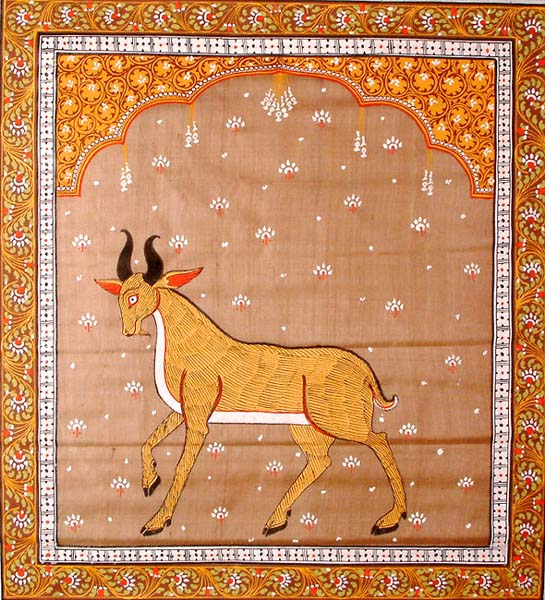
\includegraphics[width=0.5\textwidth]{pics/Aries.png}
 \end{figure}
 

Hindu Drawing of Aries as the Ram
Aries as the Ram is headstrong, assertive, forward movement, determined but obstinate.


 \begin{figure}[H]
 \centering
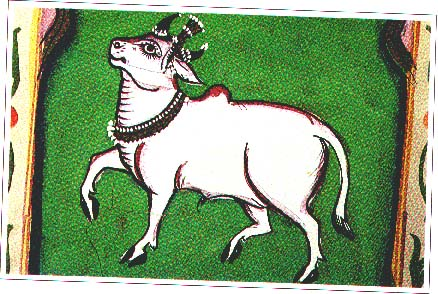
\includegraphics[width=0.5\textwidth]{pics/Taurus.png}
 \end{figure}

Hindu Drawing of Taurus as Bull
Taurus as the bull is strong, steady, creative, earthly and fixed.



 \begin{figure}[H]
 \centering
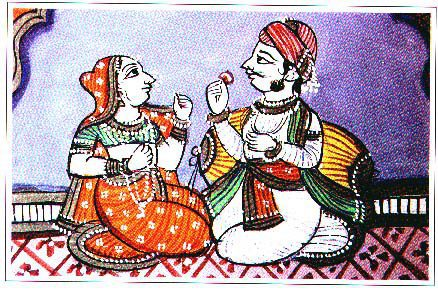
\includegraphics[width=0.5\textwidth]{pics/Gemini.png}
 \end{figure}

Hindu Drawing of Gemini
Vedic astrology regards Gemini as a male and female couple, not as twins as in western astrology.
Gemini is sensitive, volatile, communicative, relationship oriented, ambivalent.

 

\begin{figure}[H]
 \centering
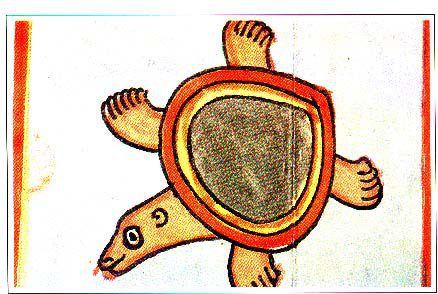
\includegraphics[width=0.5\textwidth]{pics/Cancer.png}
 \end{figure}

 

Hindu Drawing of Cancer as Crab
Cancer as a crab is often hard to understand for the sign of the Moon.
Shows the indrawn nature of lunar emotions but that can also have a power of expression.



 \begin{figure}[H]
 \centering
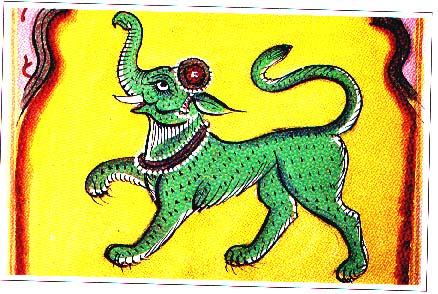
\includegraphics[width=0.5\textwidth]{pics/Leo.png}
 \end{figure}

Hindu Drawing of Leo
Combines Elephant and Lion as sign of Royalty.
Leo is warm, expressive, guiding, leading, but potentially dominating and overpowering.

 
\begin{figure}[H]
 \centering
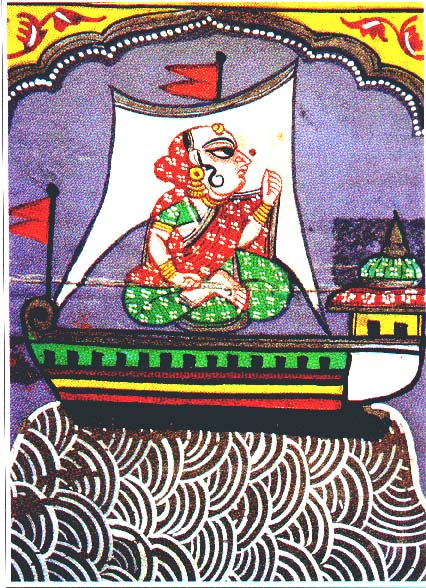
\includegraphics[width=0.5\textwidth]{pics/Virgo.png}
 \end{figure}


 

Hindu Drawing of Virgo
Vedic astrology sees Virgo as a young girl and often a woman overall.
Virgo has both manual and mental skills, is creative, sensitive, vulnerable, yet focused.

 
\begin{figure}[H]
 \centering
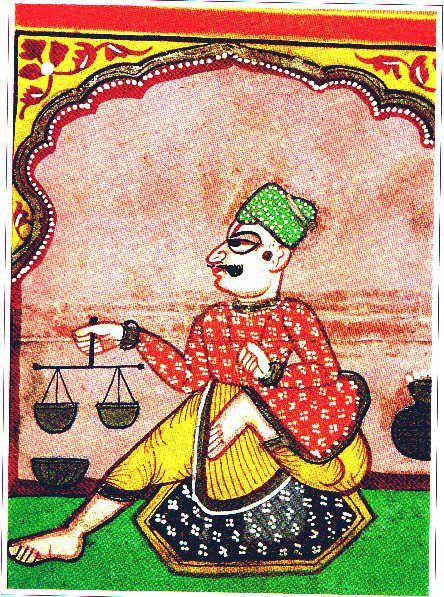
\includegraphics[width=0.5\textwidth]{pics/Libra.png}
 \end{figure}


 

Hindu Drawing of Libra
Merchant Weighing Scales
Libra is concerned with balance, harmony, commerce, communication, both on outer and inner levels.

 

\begin{figure}[H]
 \centering
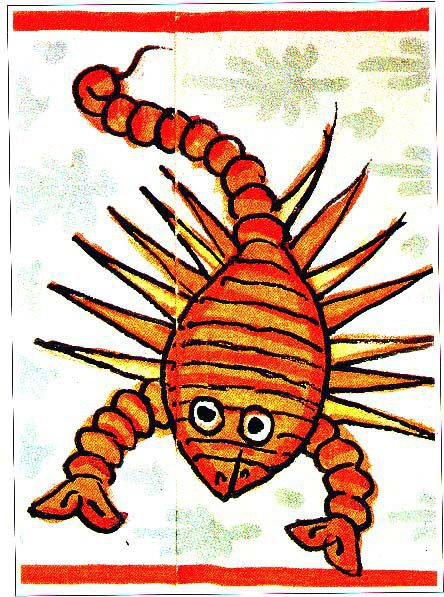
\includegraphics[width=0.5\textwidth]{pics/Scorpio.png}
 \end{figure}

 

Hindu Drawing of Scorpio

Scorpio like the literal serpent has poison in its tail and connects to deep emotional, occult and spiritual energies.


\begin{figure}[H]
 \centering
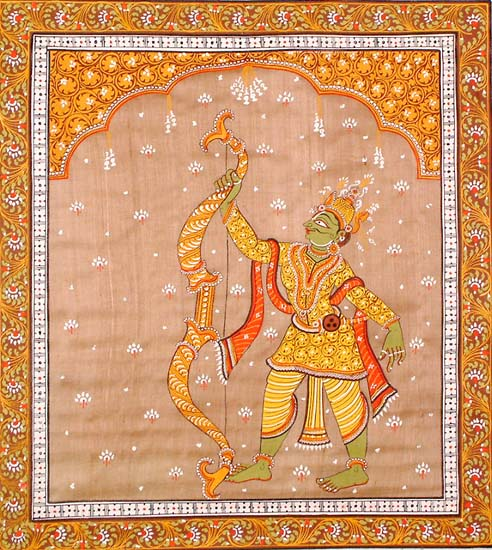
\includegraphics[width=0.5\textwidth]{pics/Sagitarius.png}
 \end{figure}


Hindu Drawing of Sagittarius
As the Bowman
Sagittarius relates to law, dharma, the police, army, gurus, and gives focus.

 

\begin{figure}[H]
 \centering
\includegraphics[width=0.5\textwidth]{pics/Capricorn.png}
 \end{figure}

 

Hindu Drawing of Capricorn
Sometimes a crocodile but other times a mountain goat is used for Capricorn.
Represents the ability to move on Earth and scale its heights but with effort and challenges.

 

\begin{figure}[H]
 \centering
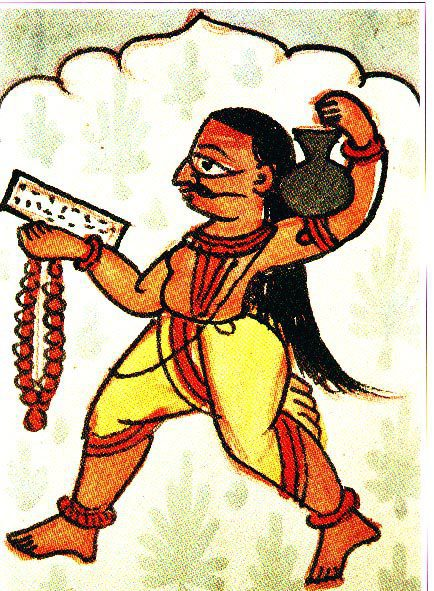
\includegraphics[width=0.5\textwidth]{pics/Aquarius.png}
 \end{figure}

Hindu Drawing of Aquarius
As a man carrying a Water Pot
The water pot is wisdom, the cosmic space, spiritual sensitivity, humanism.

 


\begin{figure}[H]
 \centering
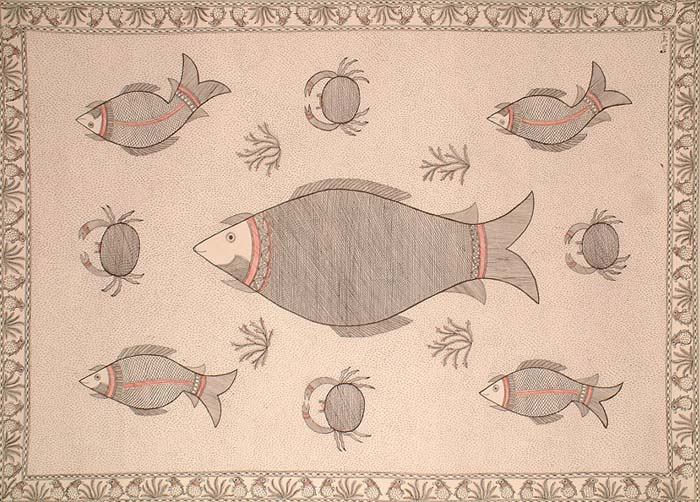
\includegraphics[width=0.5\textwidth]{pics/Pisces.png}
 \end{figure}
 

Hindu Drawing of Pisces as the Fish
The fish indicates absorption, mergence, introversion, intuition and completion.



 

COURSE WORKBOOK FOR EXAMINATION OF SOUTH AND NORTH INDIAN VEDIC CHARTS

The course Workbook, which is supplementary to the other three course volumes, is also referred to in these lessons, as we have already noted. It comes after the other three course volumes in the course index. Just scroll down to find it.

For this particular lesson, once you have completed the lesson material, please examine the first lesson of the Workbook, particularly if you do not know how to read North and South Indian charts and their differences, which the Workbook provides examples for. It teaches you how to read both types of charts. 
\newpage

\section{FOUNDATIONS OF VEDIC ASTROLOGY 2 
Houses, Nakshatras and Planetary Aspects}

In this lesson we continue with basic factors of Vedic Astrology. We summarize the main points in the lesson but have supplementary reading as well. This lesson’s prime topics will be Houses, Planetary Aspects and Nakshatras, but we will begin with additional factors of Planet and Sign Relationship.

 

Numbering of topics continues from the previous lesson (page numbers continue from the book Astrology of the Seers). Again we are introducing these topics, which will be explored in more detail as the course proceeds. Make sure here to get  basic familiarity with the terms and concepts involved. You might want to start with your own birthchart in this examination of chart factors.

 Again in this lesson there will be no lesson tests, study exercises or assignments as the lesson itself requires a lot of examination.

 

\subsection{FURTHER INDICATIONS OF THE PLANETS RELATIVE TO THE SIGNS
SIGNS OF EXALTATION AND DEBILITY }(Astrology of the Seers 103-104)

 

Planets do best when located in their signs of exaltation and suffer in their signs of debility. This is a very important consideration and the basis of certain calculations of planetary strength and weakness. Debility positions are opposite exaltation.

 

\begin{enumerate}
\item[*] Sun is exalted in Aries and debilitated in Libra, exact point 10 degrees.
\item[*] Moon is exalted in Taurus and debilitated in Scorpio, exact point 3 degrees.
\item[*] Mars is exalted in Capricorn and debilitated in Cancer, exact point 28 degrees.
\item[*] Mercury is exalted in Virgo and debilitated in Pisces, exact point 15 degrees.
\item[*] Jupiter is exalted in Cancer and debilitated in Capricorn, exact point 5 degrees.
\item[*] Venus is exalted in Pisces and debilitated in Virgo, exact point 27 degrees.
\item[*] Saturn is exalted in Libra and debilitated in Aries, exact point 20 degrees.
\item[*] Rahu and Ketu are not always given signs of exaltation and debility.
 \end{enumerate}

\subsubsection{Mulatrikona Signs for Planets}

 

Vedic astrology has the special concept of Mulatrikona or root trine, indicating other special places in which planets are powerful. These are mainly in the odd-numbered or positive sign that they rule. Mercury is exceptional in that Virgo is a sign that it rules, that it is exalted in, and that it has its Mulatrikona in. These locations give special power to the planet but not as much as exaltation.

 

\begin{enumerate}
\item[*] Sun – Leo, 4-20 degrees
\item[*] Moon – Taurus, 4-20 degrees
\item[*] Mars – Aries, 00-12 degrees
\item[*] Mercury – Virgo, 16-20 degrees
\item[*] Jupiter – Sagittarius, 00-10 degrees
\item[*] Venus – Libra 0-15 degrees
\item[*] Saturn – Aquarius, 00-20 degrees
  \end{enumerate}

Memorize the points of exaltation and debility and Mulatrikona positions for each planet, both in terms of signs and degrees. This is very important as planets gain strength towards their point of exaltation and lose it towards their point of debility. There are rules of cancellation of debility as well that we will examine later in the course.

 

\subsection{PLANETARY FRIENDSHIP AND ENMITY }(Astrology of the Seers 104-106)
 

Learn to determine planetary friendship and enmity along both natural status (unchanging) and temporal status (changing according to house location in a chart). Note that while Vedic Software will determine this for you, such basic information should be something you can calculate yourself.

 

\subsubsection{Natural Planetary Friendship and Enmity}

 

Be familiar with the two main natural groups of natural friends and enemies.

Sun, Mars, Moon, and Jupiter versus \\
Mercury, Venus and Saturn
 

Planets in the same camp will be natural friends, like Sun, Mars, Jupiter and Moon for one camp, or Mercury, Venus and Saturn for the other. Planets in different camps will be natural enemies, like Sun and Mercury, or Mars and Venus. This is a very important factor.

 

\subsubsection{Temporal or Temporary Planetary Friendship and Enmity}

 

The rule for temporal friends and enemies is also simple, but does require special calculation from the actual birth chart. It reflects the house positions of the individual chart, and is not an overall planetary rule like natural friendship and enmity. These house positions will be explained in greater detail below.

 

Planets located in houses 2,3, 4 or 10, 11, 12, from a given planet’s location will be temporal friends.\\
Planets located in the same house as a given planet or in houses 5-9 from it become temporal enemies.
 

Both natural and temporal friendship and enmity can be combined for a composite indication. Note that most Vedic software will make this calculation for you. Planets do better if located in friendly signs and suffer if located in unfriendly signs. This is something you should always examine in every chart at an initial phase of interpretation. We will examine this factor in detail later in this section of the course.

 

\subsection{3. THE TWELVE HOUSES} (Astrology of the Seers, Chapter 7, the Houses: Domains of Planetary Action, pages 111-144)


The houses (bhavas) are perhaps the most important factor in Vedic astrology and must be clearly understood in qualities. The signs reflect more the individual nature or character, while the houses reflect more our outer manifestation and external life affairs. Become capable of explaining the fields of life that relate to each house.

Lesson 6 will go into great detail on the houses and house rulership issues, which is a topic in ints own right. Note the basics here.

 

The signs and houses correlate in meaning at a general level, with each numbered sign and house having similar indications, (though this should not be taken too far as there are differences between sign and house meanings as well):

 

Aries and first house, Taurus and second house, Gemini and third house,
Cancer and fourth house, Leo and fifth house, Virgo and sixth house.
Libra and seventh house, Scorpio and eighth house, Sagittarius and ninth house.
Capricorn and tenth house, Aquarius and eleventh house, Pisces and twelfth house.
 

For example, the first house will reflect the fiery and assertive qualities of Aries, the second house will reflect the earthy and possessive aspects of Venus, the third house will address communication and expression issues like Gemini, the fourth house will cover mind and emotions like Cancer, the fifth house will cover creative intelligence like Leo, the sixth house will deal with health and disease like Virgo, the seventh house will deal with relationship like Libra, the eighth house will deal with secret and occult issues like Scorpio, the ninth house will deal with dharma like Sagittarius, the tenth house will indicate public work and impact like Capricorn, the eleventh house will address social issues like Aquarius, and the twelfth house will address spiritual issues like Pisces.

 

When the same number house and sign are influenced, the result will be stronger. For example, if a malefic planet like Mars afflicts the ninth sign Sagittarius and the ninth house, there is a greater danger of injury to the hips represented by these factors. If a benefic like Jupiter aspects the fifth sign Leo and the fifth house, it will indicate better past life karma. This is a common principle fo chart interpretation.

 

Western and Vedic astrology usually look at the houses with the same general interpretations, like the seventh house and relationship, but there are some variations. For example, the third house in Vedic is more a martial house indicated by Mars, whereas in western is more Mercurial, lie the third sign Gemini. The ascendent or first house is not a martial house like the first sign Aries but relates more to the Sun as the life energy of the person. These factors will also be examined more later in the course.

 

\subsubsection{Calculation of Houses}
 

There are different ways of calculating the houses (bhava), which can be by sign (rashi), by equal house system or by midheaven systems (Astrology of the Seers 113-115). Houses can be determined:

 

\begin{enumerate}
\item[] 1) By sign, or Equal Sign System – each sign starting with the Ascendant will refer to one house, regardless of the degree of the Ascendant or the planets within it.

\item[] 2) By 30 degree sections starting with the Ascendant or Equal House System. So if for example 10 degrees of Taurus is rising, the region 15 degrees around it will mark the first house, or from 25 Aries to 25 Taurus, with the other houses following in order, the second house as 25 Taurus to 25 Gemini and so on.

\item[] 3) By dividing up the area between the Ascendant and the Midheaven, or Midheaven systems like Sripati or Placidus. Midheaven is a special point that varies by the latitude of the place of birth. The Midheaven is not always 90 degrees from the Ascendant. So if we use the Midheaven as the cusp of the tenth house, we will need to divide up the difference into the houses in an unequal matter. This can be done automatically by current software programs by selecting such house system options.
\end{enumerate}
 

As a special note, Western and Vedic astrology interpret house cusps differently, Vedic astrology makes the cusp the middle of the house , while Western astrology makes it the the beginning of the house, though both regarding the cusp as the most powerful part of the house.

 

\subsubsection{Houses from the Moon}

 

Vedic astrology examines houses from the Moon as well as from the Ascendant. The Moon is a second ascendant or an ascendant in its own right. Houses from the Moon show more how the planets affect our feelings and personal happiness, extending to our social image, while positions relative to the Ascendant relate more to outer factors in the material world and how we are placed relative to the public. Generally we weigh the Ascendant as 2/3 in value and the Moon as Ascendant as 1/3 in value. But sometimes the weight of planetary placements and aspects will favor the Moon.

 

This means that if the same house from the Moon and the Ascendant is affected, the results will be stronger for the issues involved. For example, if the fifth house, which governs children, is afflicted from both the Ascendant and the Moon, say by aspects of Saturn and Mars, difficulties with children is more likely.

 

\subsubsection{Referred Houses}

 

We can turn any house into the Ascendant for that person or factor indicated by the specific house examined, what are called “referred houses” (bhavat-bhavm). For example, we can turn the seventh house the Ascendant and use it for reading the condition of the marriage partner from there. In Vedic astrology the house dial is a like a revolving wheel and can be placed in different parts of the chart relative to different considerations. The normal Ascendant or Rashi chart is the main dial but other secondary factors can also be read. We will examine this factor in greater detail in the Workbook.

 

\subsection{HOUSE QUALITIES} (Astrology of the Seers, pages 117-120)

 

There are three basic qualities of the houses, which are of great importance.\\
Angular or Kendra (1, 4, 7, 10)\\
Succedent  (2, 5, 8, 11)\\
Cadent (3, 6, 9, 12) 
 

Planets are usually stronger placed when kendra or angular positions (Houses 1,4, 7, 10). They are weak when placed in cadent houses (Houses 3, 6, 9, 12) They are of moderate strength when placed in  succedent houses (Houses 2,5,8, 11) These qualities roughly parallel the three qualities of the signs as cardinal, fixed and mutable (moveable, fixed and dual). It is a key consideration in looking at the chart for planetary strengths and weakness.

 

\subsubsection{Additional House Groupings}

Trine (trikona) house locations (1, 5, 9) are also auspicious and powerful, for all aspects of the life and character of a person.\\
Upachaya or increasing house locations (3, 6, 10, 11), as special distinction of Vedic astrology  are good for malefics and give powers of competition, endurance and resistance, gaining more power with age.\\
Apachaya or decreasing house locations (1, 2, 4, 7, 8) houses bring initial benefits but cause planets to lose their strength and value over time.\\
Bad or difficult house locations (6, 8, 12), Duhsthanas are the worst positions in the chart, particularly house 8. All planets weak are if located in these positions, particularly benefics.\\
The houses like the signs (following house-sign correspondence principles) also divided according to to the four elements of Earth 2,6,10), Water (4,8,12), Fire (1,5,9) and Air (3,7,11). For example, the first house like the first sign Aries has a fiery quality.\\
The houses area divided according to the four aims of life as dharma or vocation (houses 1,5,9), artha or prosperity (houses 2,6,10), kama or happiness (houses 3,7,11) and moksha or liberation (houses 4,8, 12).
 

Examine the Description of the Houses in the Astrology of the Seers  (121-128). Learn how to describe each house. Become intimate with its qualities, connections and associations. The houses are the key to chart interpretation. You should know the house qualities as clearly as you know those of the signs.

 

\subsubsection{The natural significators of each house:}

These are special planetary significators unique to Vedic astrology. Some houses have more than one depending upon the factors involved.
Sun and the first house\\
Jupiter and the second house\\
Mars and the third house\\
Moon and the fourth house\\
Jupiter and the fifth house\\
Saturn and Rahu and the sixth  house\\
Jupiter and Venus and the seventh house\\
Saturn and the eighth house\\
Jupiter and Sun and ninth house\\
Sun and Mercury and the tenth house, Mars is also strong there\\
Jupiter and the eleventh house\\
Saturn and Ketu and the twelfth house
 

Jupiter is the significator of several different houses (2, 5, 7, 9, 11). Saturn signifies several houses (6, 8, 12) or all the difficult houses or duhsthanas. Remember that if the natural significator of a house is weak, the house is also likely to be weak.

 

\subsection{PRINCIPLES OF HOUSE RULERSHIP} (Astrology of the Seers, pages 131-142)

 

House rulership, meaning the planet that rules a particular house in a given chart, is one of the most important principles of Vedic astrology and the basis of most interpretations and predictions. Many Vedic astrological combinations or yogas are defined by house rulership (like the ruler of the first house located in the sixth house and the ruler of the sixth house located in the first house, which is a combination that causes disease).

 

Examine the principles of house rulership and see how the meaning of planets changes relative to each ascendant according to the houses that they rule (also called the “temporal status” of a planet). But note that this is covered in a special lesson of its own for more detail.***

 

The complication is that the planets, except Sun and Moon, rule over two houses, one which may have good effects and one that may be difficult. The planet will give the results of both houses it rules, though at different times and different ways. For example, in the case of an Aries ascendant, Mars will rule both the first house (Aries) and the eighth house (Scorpio). Mars rulership of the eighth house will bring in some negative energies, while overall the ruler of the first is regarded as a positive planet.

 

When a planet rules both an angle (1, 4, 7, 10) and a trine (1, 5, 9), it  called a Raja Yoga planet . This gives great power, influence and success in life. Some Ascendants have one planet that does this, like Saturn ruling houses 4 and 5, for Libra Ascendant. Yet Raja Yogas can be created by two planets, if one rules and angle and the other rules a trine.

 

Note that planets function according to the nature of the houses that they rule as well as according to their natural qualities. For example, even when a natural malefic like Saturn rules good houses, it can still cause some difficulties, yet as a Yoga Karaka for Libra ruling houses 4 and 5, its overall effects will be quite good. Never forget to look at the houses they are connected to before judging their effects.

\subsubsection{4. THE TWENTY-SEVEN NAKSHATRAS} (Astrology of the Seers 108-109)
 

At this point we are just introducing the 27 Nakshatras by name and position.  Learn the 27 Nakshatras by name and their positions in the zodiac (the 13 degree 20 minute section that each rules). In the long-term try to memorize them. What you need to know at this point is only introductory. The third section of the course will examine the Nakshatras in great detail and several lessons.

THE 27 NAKSHATRAS\\
ASHWINI, 00 00—13 20 Aries:  “The horses head”. It originally represented the head of the sacrificed horse that symbolized the Sun, the year and the beginning of the cycle of time.Deity—the Ashwins, the twin horsemen (like Castor and Pollux of the Greeks).\\
BHARANI, 13 20—26 40 Aries:  “The bearers”. It is symbolized by the female reproductive organ. Deity—Yama, the God of death and immortality.\\
KRITTIKA, 26 40 Aries—10 00 Taurus:  “The razor”, which is also its symbol. It corresponds to the stars of the Pleiades, the small cluster of six stars in Taurus. Deity—Agni, the God of fire.
ROHINI, 10 00—23 20 Taurus:  “The red or ruddy female deer or antelope”, from its prime star, red Aldeberan or Alpha Taurus. Deity—Prajapati, the lord of creation.\\
MRIGASHIRAS, 23 20 Taurus—06 40 Gemini:  “The antelopes head”, or the head of the sacrificed wild animal or creator God. Now it is related to the head of the constellation Orion, but originally consisted of the three stars in his belt. Deity—Soma, the God of immortality.\\
ARDRA, 06 40—20 00 Gemini:  “The moist”, marked by the red star Betelgeuse, Beta Orion. Deity—Rudra (Shiva), the God of the storm and the bowman or hunter.\\
PUNARVASU, 20 00 Gemini—03 20 Cancer:  “Return of the light”, marked by Castor and Pollux, Alpha and Beta Gemini. Deity—Aditi, the Mother of the Gods who is sometimes identified with the earth but mainly represents the sky.\\
PUSHYA, 03 20—16 40 Cancer:  “The nourisher”, Deity—Brihaspati, the teacher of the Gods. Deity of the planet Jupiter.\\
ASHLESHA, 16 40—30 00 Cancer:  “The serpent”, Deity—Sarpa, the Serpent in all forms.\\
MAGHA, 00 00—13 20 Leo:  “the beneficent”, marked by Regulus, Alpha Leo, Deity—the Fathers or Ancestors.\\
PURVA PHALGUNI, 13 20—26 40 Leo:  “The earlier fig tree”, Deity—Bhaga, the Sun of bliss.\\
UTTARA PHALGUNI, 26 40 Leo—10 00 Virgo:   “The later fig tree”, marked mainly by Denebola, Beta Leo, Deity—Aryaman, the Sun as the beloved, the friend or the helper.\\
HASTA, 10 00—23 20 Virgo:  “The hand”, corresponding to the constellation Corvus. Deity—Savitar, the Sun of inspiration (Apollo).\\
CHITRA, 23 20 Virgo—06 40 Libra:  “The brilliant”, marked by the star Spica, Alpha Virgo. Deity—Twashtar, the Divine craftsman and demiurge.\\
SWATI, 06 40—20 00 Libra:  “The sword”, marked by the star Arcturus, Alpha Bootes. Deity—Vayu, the God of Air or the Wind, also Prana or the life-force.\\
VISHAKHA, 20 00 Libra—03 20 Scorpio:  “The two branches”, marked mainly by Alpha Libra. Deity—Indragni, the dual Gods of Fire and Thunder.\\
ANURADHA, 03 20—16 40 Scorpio:  “Subsequent success, following or devotion”, Deity—Mitra, the Divine friend and lord of compassion.\\
JYESHTA, 16 40—30 00 Scorpio:  “The eldest”, marked mainly by Antares, Alpha Scorpio. Deity—Indra, God of lightning and perception.\\
MULA, 00 00—13 20 Sagittarius:  “The root”, marked by the stars in the tail of Scorpio. Deity—Nirriti, the Goddess of disaster and negation.\\
PURVASHADHA, 13 20—26 40 Sagittarius:  “The earlier victory”. Deity—Apas, the Goddess of the Waters or cosmic sea.\\
UTTARASHADHA, 26 40 Sagittarius—10 00 Capricorn:  “The later victory”. Deity—Vishwedevas, the Universal Gods.\\
SHRAVANA, 10 00—23 20 Capricorn:  “The famous or renowned”, marked mainly by the star Altair, Alpha Aquila, Deity—Vishnu, the Pervador\\
DHANISHTA OR SHRAVISHTA, 23 20 Capricorn—06 40 Aquarius:  “The most wealthy or most famous”, Deity—the Vasus, the Gods of light.\\
SHATABHISHAK, 06 40—20 00 Aquarius:  “What has a hundred medicines”. Deity—Varuna, the God of the cosmic ocean or heavenly waters.\\
PURVA BHADRA, 20 00 Aquarius—03 20 Pisces:  “The earlier auspicious one”, marked mainly by Alpha Pegasus. Deity—Aja Ekapat, the one-horned goat or unicorn.\\
UTTARA BHADRA, 03 20—16 40 Pisces:  “The later auspicious one”, Deity—Ahir Budhnya, the Dragon of the depths.\\
REVATI, 16 40—30 00 Pisces:  “The rich or splendorous”, Deity—Pushan, the Sun in his protective, nourishing or fostering role, particularly relative to the Earth.\\
 

Nakshatras are a subtler division than the signs and help us understand how different parts of signs work. The main practical usage of Nakshtras is for determining planetary periods (dashas) through the Vimshottari dasha system. Yet we do consider Nakshatras as personality types, much like the Sun signs of western astrology. In addition we can judge the effects of planets relative to the Nakshatras in which they are located. Sometimes the Nakshatras are called Lunar Mansions or Lunar Asterisms reflecting their connection with the Moon, but they do have other connections as well and we do not like to use these terms.

 

 



 

\subsection{5. PLANETARY ASPECTS AND ASSOCIATIONS} (Astrology of the Seers, Chapter 9, pages 145-160)
 

Aspects are key factors in astrological interpretation and are highly emphasized in western astrology, where they are calculated with much precision. Planetary aspects or drishtis (meaning views or sights) are also important in Vedic astrology but calculated different than in western astrology, and in a more general manner. The Vedic view of aspects are largely sign based, from that of Western Astrology is degree based. Remember these differences between Western and Vedic usage and determination of planetary aspects. In addition Vedic astrology has other tools like friendship and enmity to judge planetary relations even when specific aspects may not exist. It is not as aspect centered as is western astrology.

 

Learn the major aspects of the planets as they occur by sign.

 

Each planet aspects the sign seventh from it.
For Sun, Moon, Mercury and Venus, these are the only aspects that the planets have.
For example, if the Moon is in Taurus it will aspect Scorpio as the seventh sign from it.
Each planet is also considered to have a direct relationship like an aspect with planets that it shares the same sign, which is called a conjunction.
 

\subsubsection{SPECIAL ASPECTS OF MARS, JUPITER AND SATURN}

 

Mars has additional special aspects on the fourth and eighth signs from its location.
Jupiter has additional special aspects on the fifth and ninth signs from its location.
Saturn has additional special aspects on the third and tenth signs from its location.
 

These special aspects give special power to these three planets, which relate to fire and Pitta (Mars), water and Kapha (Jupiter) and air and Vata (Saturn).

 

\subsubsection{Rahu and Ketu}

Sometimes Rahu and Ketu are given trinal aspects like Jupiter, but this is a secondary opinion. The Rahu-Ketu axis in the chart, including the opposite signs in which it occurs, has its importance in astrological interpretation as well. It forms important Yogas like Kala Sarpa.

 

\subsubsection{Aspects in Divisional Charts}

Note that the same aspects can be used in divisional charts like the Navamsha, though some Vedic astrologers do not use them. We find them to be very useful and always examine them.

 

\subsubsection{Determination of Aspects by Sight}

You should be able to determine these major aspects in the Vedic chart by sight alone, by merely looking at the chart (this is the basis of memorizing charts). That is why there is often  no table of aspects given on the Vedic chart as there is in most western charts. Such simple by sign aspects are easier to see than the degree aspects of western astrology. Yet we should note that when aspects are close by degrees, particularly conjunction and opposition (same sign or opposite sign), they may be stronger in their effects.

 

\subsubsection{Sambandha or Full Relationship between Planets}

Note the principles for determining Sambandha, or complete association between planets, which consists of either conjunction (same sign), mutual full aspect, or exchange of signs like Mars in Gemini ruled by Mercury and Mercury in Scorpio ruled by Mars.. This brings planets into a very close relationship.

 

\subsubsection{Combust Planets}

Planets become combust (burned up by being too close to the Sun). Generally any planet in the same sign with the Sun may likely be combust, generally within fifteen degrees of the Sun.  Generally combust for planets close to the Sun as Mercury and Venus, is not as severe, as they are always not far from the Sun. Of these two combust Venus is the worst. Meanwhile, combust for the outer planets Mars, Jupiter and Saturn is more severe. Combust Saturn is usually the most difficult.

Combustion also affects house ruler. For example, a combust Ascendant Lord can have problems for a person, particularly in terms of health. A combust fourth lord may not bode well for the mother, by way of another example.

 

\subsubsection{Planetary War}

Planetary war (graha yuddha) is generally said to occur if planets are in a conjunction of less than one degree. Generally the planet with the lower number of degrees and minutes will win the war, but some variant opinions are out there. The planet that loses the war becomes much weaker.

 

\subsubsection{Separative Planets}

The Sun, Saturn, Rahu and the lord of the twelfth house (and sometimes Mars) are considered to be separative planets and negate or remove us from the qualities of the house or planet they influence. On the other hand, Moon, Venus and Jupiter tend to strengthen the positive qualities of the house or planet they influence. These rules are extensions of the natural benefic or malefic statys of planets.

Planets or houses with natural malefic planets on either side suffer, called being “hemmed in between malefics” or Papakartari Yoga.\\
Planets or houses with natural benefic planets on either side do well, called being “hemmed in between benefics” or Shubhakartari Yoga.\\
Always look to the disposition of planets around any given planet, mainly in adjacent signs, which can be as important as aspects. Do not examine the planet in a single sign only. Consider not only aspects but planetary proximity, friendships and enmities.

 

\subsubsection{Weight of Planetary Aspects}

Note the weight of aspects in a chart, particularly relative to natural benefic and malefic planets, including which planets have the most influence on the chart.

See which planets or houses have the most aspects upon them in a given chart. As Mars, Jupiter, and Saturn have special aspects they become particularly powerful and generally indicate the fire (Pitta), water (Kapha) and air (Vata) factors in the chart.

 

\subsection{PLANETARY YOGAS}
 

Yogas are general names for combined planetary influences. They are defined in various ways relative to house or sign location, house or sign rulership, and aspects, or even special patterns of planetary influence. The concept of yogas is broader and diverse and can be more important than aspects in Vedic astrology but may include them. Yoga are the culminating and most important aspect of chart interpretation and are the subject of extensive analysis in advanced studies in Vedic astrology. Their are entire books on this subject.

 

Very important and a good place to start are Mahapurusha Yogas, formed by planets being located in an angle from the Ascendant or Moon as well as in their own sign or exalted, does not include Sun or Moon. These are important for determining planetary types of people which are often created by these planetary Yogas.

 

Yogas affecting the Moon are important as the Moon is like another Ascendant. The Moon does best with other planets, particularly benefics, with or around it. It suffers from isolation, which can lead to debility and depression. Yet many other Yogas exist. We will discuss these in greater detail later in the course as they are very important overall.
\newpage


\newpage



% ------------------------------------------------------------------------------

\end{document}
